\input{Carta3.tex}

\usepackage{hyperref}
\usepackage{setspace}
\usepackage{lscape}
\usepackage{dcolumn}
\usepackage{rotating}
\renewcommand{\titulodoc}{Compendio SAN}


\renewcommand{\contentsname}{Contenidos}

\begin{document}
\renewcommand{\thepage}{\roman{page}}
\clearpage

$\ $
\vspace{14.5cm}

\noindent\begin{tabular}{p{0.9cm}p{6.8cm}}
& 2016.$\,$ Guatemala, Centro América \\
&\Bold Instituto Nacional de Estadística\\[-0.4cm]
&\color{blue!50!black}\url{www.ine.gob.gt}\\[0.9cm]
\end{tabular}\\
\noindent\begin{tabular}{p{0.9cm}p{6.8cm}}
& Está permitida la reproducción parcial o total de los contenidos de este documento con la mención de la fuente. \\[0.5cm]
 
& Este documento fue elaborado empleando  {\Sans R}, Inkscape y {\Logos \XeLaTeX}.\\
\end{tabular} 
\pagestyle{estandar}

\clearpage


%	\includepdf{portadaazul.pdf}
	
	\clearpage
	\newpage $\ $
	\newpage $\ $
$\ $
\vspace{7cm}

\begin{center}
\Bold \LARGE COMPENDIO ESTADÍSTICO DE\\
SEGURIDAD ALIMENTARIA Y NUTRICIONAL 2015
\end{center}
\cleardoublepage
\pagestyle{estandar}
%
%$\ $
%\vspace{0.0cm}
%
%\begin{center}
%{\Bold \LARGE AUTORIDADES}\\[1cm]
%
%
%{\Bold \large \color{color1!89!black} JUNTA  DIRECTIVA} \\[0.4cm]
%
%
%{\Bold Ministerio de Economía}\\
%Titular: Rubén Estuardo Morales Monroy\\
%Suplente: Abel Francisco Cruz Calderón\\[0.4cm]
%
%
%{\Bold Ministerio de Finanzas}\\
%Titular: Julio Héctor Estrada\\
%Suplente: Victor Manuel Martínez Ruiz\\[0.4cm]
%
%
%{\Bold Ministerio de Agricultura, Ganadería y Alimentación}\\
%Titular: Mario Méndez Montenegro\\
%Suplente:  Rosa Elvira Pacheco Mangandi\\[0.4cm]
%
%
%{\Bold Ministerio de Energía y Minas}\\
%Titular: Juan Pelayo Castañón\\
%Suplente: César Roberto Velásquez Barrera\\[0.4cm]
%
%
%{\Bold Secretaría de Planificación y Programación de la Presidencia}\\
%Titular: Miguel Ángel Moir Mérida\\
%Suplente: Edna Abigail Álvarez\\[0.4cm]
%
%
%{\Bold Banco de Guatemala}\\
%Titular: Julio Roberto Suárez Guerra\\
%Suplente: Sergio Francisco Recinos Rivera\\[0.4cm]
%
%
%
%{\Bold Universidad de San Carlos de Guatemala}\\
%Titular: Murphy Olimpo Paiz\\
%Suplente:  Óscar René Paniagua \\[0.4cm]
%
%
%{\Bold Universidades Privadas}\\
%Titular: Miguel Ángel Franco de León\\
%Suplente: Ariel Rivera Irías\\[0.4cm]
%
%
%{\Bold Comité Coordinador de Asociaciones\\ Agrícolas, Comerciales, Industriales y Financieras}\\
%Titular: Juan Raúl Aguilar Kaehler\\
%Suplente:  Oscar Augusto Sequeira García\\[0.8cm]
%
%
%{\Bold \large \color{color1!89!black} GERENCIA}\\[0.2cm]
%Gerente: Néstor Mauricio Guerra Morales.\\
%Subgerente Técnico: Jaime Roberto Mejía Salguero\\
%Subgerente Administrativo Financiero: Orlando Roberto Monzón Girón\\
%
%
%\end{center}

\clearpage

$\ $
\vspace{1cm}

\begin{center}
{\Bold \LARGE AUTORIDADES INSTITUCIONALES}\\[2cm]

{\Bold \large \color{color1!89!black} Dirección de Censos y Encuestas}\\[0.2cm]
Carlos Enrique Mancía Chúa\\[0.8cm]


{\Bold \large \color{color1!89!black} Dirección de Índices y Estadísticas Continuas}\\[0.2cm]
Luis Eduardo Arroyo Gálvez\\[0.8cm]

{\Bold \large \color{color1!89!black} Dirección Administrativa}\\[0.2cm]
Edgar Rolando Elías Pichillá\\[0.8cm]

{\Bold \large \color{color1!89!black} Dirección Financiera}\\[0.2cm]
María Elena Galindo Rodríguez\\[0.8cm]


{\Bold \large \color{color1!89!black} Dirección de Informática}\\[0.2cm]
César Calderón Barillas\\[0.8cm]


\end{center}\cleardoublepage

%%%%%%%%%%%%%%%%%%%%%%%%%%%%%%%%%%%
\clearpage

$\ $
\vspace{1cm}

\begin{center}
	{\Bold \LARGE EQUIPO RESPONSABLE}\\[2cm]
	
	{\Bold \large \color{color1!89!black} Coordinación general:}\\[0.2cm]
Nestor Mauricio Guerra Morales – Gerente INE \\
Edwin Portillo Portillo – Sub-gerente administrativo financiero INE \\
Fredy Arizmendy Gómez Gómez – Sub-gerente técnico INE \\
Raúl Maas – Director Iarna-URL\\[0.8cm]

{\Bold \large \color{color1!89!black} Coordinación técnica y contenido:}\\[0.2cm]
Lorena Ninel Estrada – Iarna-URL\\
Haydee Azucena Barrientos Osorio– INE\\
Juan Enrique Lee Samayoa- INE\\
Luis Eduardo Arroyo Gálvez – INE\\
Gonzalo Adolfo Hernández – Sesan\\
Nora Griselda Cano Escalante– Sesan\\
Héctor Antonio Tuy - Iarna-URL\\
Jaime Luis Carrera - Iarna-URL\\[0.8cm]
%Lorena Ninel Estrada – Iarna-URL\\
%Haydeé Barrientos - INE\\
%Juan Lee - INE\\
%Luis Eduardo Arroyo Gálvez - INE\\
%Gonzalo Hernández - Sesan\\
%Nora Cano - Sesan\\[0.8cm]
{\Bold \large \color{color1!89!black} Recopilación de datos:}\\[0.2cm]

Renato Vargas – Iarna-URL\\
Vivian Guzmán – Iarna-URL \\
Hugo Allan García - Iarna-URL \\
Fabiola Beatriz Ramírez - Iarna-URL \\[0.8cm]

	{\Bold \large \color{color1!89!black} Edición:}\\[0.2cm]
Haydee Azucena Barrientos Osorio - INE\\
Lorena Ninel Estrada - Iarna-URL \\[0.8cm]


		
\end{center}\cleardoublepage
%\swapgeometry

%%%%%%%%%%%%%%%%%%%%%%%%%%%%%%%%%%%%%%%



\clearpage

$\ $
\vspace{1cm}

\begin{center}
	{\Bold \LARGE Oficina Coordinadora Sectorial de Estadísticas de Seguridad Alimentaria y Nutricional (OCSESAN)}\\[2cm]
	
\begin{itemize}
	\item Asociación de Investigación y Estudios Sociales (Asies)
	\item 	Asociación Nacional de Municipalidades (ANAM)
	\item 	Instituto de Investigación y Proyección sobre Ambiente Natural y Sociedad  (Iarna-URL)
	\item 	Instituto Guatemalteco de Seguridad Social (IGSS)
	\item 	Ministerio de Ambiente y Recursos Naturales (MARN)
	\item 	Ministerio de Economía de Guatemala (Mineco)
	\item 	Ministerio de Educación (Mineduc)
	\item 	Ministerio de Finanzas Públicas (Minfin)
	\item 	Ministerio de Salud Pública y Asistencia Social (Mspas)
	\item 	Ministerio de Trabajo y Previsión Social (Mintrab)
	\item 	Procuraduría de los Derechos Humanos de Guatemala (PDH)
	\item 	Secretaría de Seguridad Alimentaria y Nutricional (Sesan)
	\item 	Secretaría General de Planificación y Programación de la Presidencia (Segeplan)
	\item 	Usaid/DevTech - Programa de Monitoreo y Evaluación
	\item 	Viceministerio de Seguridad Alimentaria y Nutricional (Visan)
	\item 	Ministerio de Agricultura, Ganadería y Alimentación (MAGA)
\end{itemize}	

\end{center}\cleardoublepage
%\swapgeometry


%%%%%%%%%%%%%%%%%%%%%%%%%%%


\clearpage

$\ $
\vspace{1cm}

\begin{center}
	{\Bold \LARGE Fuentes primarias de información}\\[2cm]
	
	\begin{itemize}
			\item Banco Mundial (BM)
			\item 	Banco de Guatemala (Banguat)
			\item 	Instituto Guatemalteco de Seguridad Social (IGSS)
			\item 	Instituto Nacional de Estadística (INE)
			\item 	Ministerio de Agricultura, Ganadería y Alimentación (MAGA) – Dirección de Planeamiento (Diplan)
			\item 	Ministerio de Finanzas (Minfin) - Sistema de Contabilidad Integrada (Sicoin)
			\item 	Ministerio de Salud Pública y Asistencia Social (Mspas) - Sistema de Información Gerencial de Salud (Sigsa)
			\item 	Ministerio de Trabajo y Previsión Social (Mintrab)
			
	\end{itemize}	
	
\end{center}\cleardoublepage
%\swapgeometry




\cleardoublepage
\pagestyle{estandar}
\setlength{\arrayrulewidth}{1.0pt}





\cleardoublepage


$\ $\\[2cm]
\indent\titulo{\Bold \huge Presentación}
\addcontentsline{toc}{chapter}{Presentación}
\addtocontents{toc}{\protect\thispagestyle{estandar}}




$\ $\\[0.5cm]
\large
\indent El Instituto Nacional de Estadística 	(INE) se complace en presentar el Compendio Estadístico para Seguridad Alimentaria y Nutricional 2015, con la finalidad de contribuir a mejorar el nivel de comprensión sobre el estado de la Seguridad Alimentaria y Nutricional (SAN) y sus condicionantes en el país.

El INE como ente rector y coordinador del Sistema Estadístico Nacional (Decreto Ley 3-85 Ley Orgánica del Instituto Nacional de Estadística), impulsa diferentes iniciativas tendientes a mejorar la calidad de la estadística en SAN, así como los procesos de recopilación, procesamiento, análisis y difusión de la misma, siendo este compendio uno de estos procesos.

La información contenida en este documento se organizó en siete capítulos con sus respectivos indicadores y sub-indicadores. El primer capítulo es una caracterización poblacional del país. Los siguientes cinco capítulos corresponden específicamente a las dimensiones de seguridad alimentaria y nutricional, y son: a) Disponibilidad de alimentos, b) acceso a los alimentos, c) consumo de los alimentos, d) utilización biológica de los alimentos, y e) situación y atención a la desnutrición/malnutrición. El último capítulo corresponde a  inversión pública en seguridad alimentaria y nutricional. 

Las dimensiones, indicadores y sub-indicadores en que se basó el compendio fueron socializados durante las reuniones ordinarias y extraordinarias de la Ocsesan, por lo que los representantes de las instituciones miembros que asistieron tuvieron la oportunidad de brindar retroalimentación. Los cuadros con la información estadística, de la cual se derivan las gráficas, se encuentran disponibles en la versión electrónica del compendio SAN, en formato xlsx.

Asimismo, mediante un proceso de retroalimentación usuario-productor, el INE espera recibir comentarios acerca de este trabajo, con el fin de mejorar continuamente la información presentada, así como mejorar los procesos que engloban la generación, procesamiento y difusión del Compendio Estadístico SAN 2015.


$\ $

\cleardoublepage
	


\indent\titulo{Agradecimientos}
\addcontentsline{toc}{chapter}{Agradecimientos}
\addtocontents{toc}{\protect\thispagestyle{estandar}}
\\


Detrás de este esfuerzo de integración, procesamiento, análisis y difusión de la información, hay una cantidad de instituciones representadas por profesionales y técnicos, que participaron en la producción del Compendio Estadístico en Seguridad Alimentaria y Nutricional (SAN) 2015, en forma directa o indirecta.

El INE deja constancia de su agradecimiento a las siguientes entidades: La Secretaría de Seguridad Alimentaria y Nutricional (Sesan), el Sistema de Información Gerencial de Salud (Sigsa) del Ministerio de Salud Pública y Asistencia Social (Mspas), El Ministerio de Finanzas Públicas (Minfin), la Secretaría General de Planificación y Programación de la Presidencia (Segeplan), el Ministerio de Educación (Mineduc), el Viceministerio de Seguridad Alimentaria y Nutricional (Visan), y la Dirección de Planeamiento (Diplan) del Ministerio de Agricultura, Ganadería y Alimentación (MAGA), el Ministerio de Ambiente y Recursos Naturales (MARN), la Procuraduría de los Derechos Humanos de Guatemala (PDH), el Instituto Guatemalteco de Seguridad Social (IGSS), el Ministerio de Economía de Guatemala (Mineco), la Asociación de Investigación y Estudios Sociales (Asies), el Ministerio de Trabajo y Previsión Social (Mintrab), y la Asociación Nacional de Municipalidades (Anam).

Asimismo, se agradece el apoyo del Instituto de Investigación y Proyección sobre Ambiente Natural y Sociedad (Iarna) de la Universidad Rafael Landívar (URL), y a DevTech Systems por el apoyo técnico y financiero derivado del sub-contrato No. 1096-SC-13-001-00.\\[16mm]



%%%%%%%%%%%%%%%%%%%%%%%%%%%
\newpage
	$\ $\\[-1cm]
 \textcolor{color2}{\Huge Acrónimos y abreviaturas}\\
	\normalsize	$\ $\\
\begin{center}\fontsize{3.8mm}{1.4em}\selectfont \setlength{\arrayrulewidth}{0.7pt}
	$\ $\\[-1.5cm]
	$\!$\begin{tabular}{p{4.3cm}l}	\hline
	ANAM	&	Asociación Nacional de Municipalidades	\\
\rowcolor{color1!5!white}	Asies	&	Asociación de Investigación y Estudios Sociales	\\
	Banguat	&	Banco de Guatemala	\\
\rowcolor{color1!5!white}	Cacif	&	Comité Coordinador de Asociaciones Agrícolas, Comerciales, Industriales y Financieras	\\
	CMA	&	Cumbre Mundial sobre la Alimentación	\\
\rowcolor{color1!5!white}	Diplan	&	Dirección de Planeamiento	\\
	Encovi	&	Encuesta Nacional de Condiciones de Vida	\\
\rowcolor{color1!5!white}	ENEI	&	Encuesta Nacional de Empleo e Ingresos	\\
	Ensmi	&	Encuesta Nacional de Salud Materno Infantil	\\
\rowcolor{color1!5!white}	FAO	&	Organización de las Naciones Unidas para la Alimentación y la Agricultura, por sus siglas en inglés	\\
	FIDA	&	Fondo Internacional de Desarrollo Agrícola	\\
\rowcolor{color1!5!white}	GHI	&	Índice del Hambre Global, siglas en inglés	\\
	GSARS	&	Estrategia Global para el Mejoramiento de las Estadísticas	\\
	\rowcolor{color1!5!white}Iarna	&	Instituto de Agricultura, Recursos Naturales y Ambiente	\\
		IDH	&	Índice de Desarrollo Humano\\
\rowcolor{color1!5!white}	Ifpri	&	Instituto de Investigación de Política Alimentaria	\\
	IGSS	&	Instituto Guatemalteco de Seguridad Social	\\
		\rowcolor{color1!5!white} INE	&	Instituto Nacional de Estadística\\
	MAGA	&	Ministerio de Agricultura, Ganadería y Alimentación	\\
	\rowcolor{color1!5!white}MARN	&	Ministerio de Ambiente y Recursos Naturales	\\
	MEM	&	Ministerio de Energía y Minas	\\
	\rowcolor{color1!5!white}Mineco	&	Ministerio de Economía de Guatemala	\\
	Mineduc	&	Ministerio de Educación	\\
	\rowcolor{color1!5!white}Minfin	&	Ministerio de Finanzas Públicas	\\
	Mspas	&	Ministerio de Salud Pública y Asistencia Social	\\
	\rowcolor{color1!5!white}Mintrab	&	Ministerio de Trabajo y Previsión Social	\\
	Ocsesan	&	Oficina Coordinadora Sectorial de Estadísticas de Seguridad Alimentaria y Nutricional	\\
	\rowcolor{color1!5!white} ODM	&	Objetivos del Desarrollo del Milenio	\\
	PDH	&	Procuraduría de los Derechos Humanos de Guatemala	\\
	\rowcolor{color1!5!white}PMA	&	Programa Mundial de Alimentos	\\
	PPH0	&	Plan del Pacto Hambre Cero	\\
	\rowcolor{color1!5!white}SAN	&	Seguridad Alimentaria y Nutricional	\\
	Segeplan	&	Secretaría General de Planificación y Programación de la Presidencia	\\
	\rowcolor{color1!5!white}Sesan	&	Secretaría de Seguridad Alimentaria y Nutricional	\\
	Sicoin	&	Sistema de Contabilidad Integrada (Sicoin)	\\
	\rowcolor{color1!5!white}Sigsa	&	Sistema de Información Gerencial de Salud	\\
	URL	&	Universidad Rafael Landívar	\\
	\rowcolor{color1!5!white}Usaid	&	Agencia de los Estados Unidos para el Desarrollo Internacional, siglas en inglés	\\
	Visan	&	Viceministerio de Seguridad Alimentaria y Nutricional	\\
		\hline
		&\\[-0.28cm]
		%			\multicolumn{9}{l}{\footnotesize Fuente: Informe Nacional de Desarrollo Humano (PNUD), con base en las Encuestas Nacionales de Condiciones de Vida (Encovi).}
	\end{tabular}
\end{center}



$\ $\\[1cm]
\newpage
\renewcommand{\contentsname}{Contenidos}
\tableofcontents
\clearpage
\thispagestyle{estandar}
\listofexample



\newpage
%	\tableofcontents
		\pagestyle{estandar}


\input{introduccion.tex}
\input{infoPilares.tex}
	\INEchaptercarta{Población}{La dimensión de Población reúne información sobre la caracterización poblacional de Guatemala e incluye la densidad poblacional, vivienda, pobreza y trabajo. 
		
		Esta dimensión se compone de cuatro indicadores y 8 sub-indicadores.
		
		El indicador \textbf{1.1 Población}, cuenta con cinco sub-indicadores:%\\[-.3cm] 
		
		\begin{itemize}
			\item[a)] proyecciones al 2015, %\\[-.3cm]
			\item[b)] densidad, 
			\item[c)] grupos quinquenales de edad, 
			\item[d)] población y densidad a nivel departamental, 
			\item[e)] Índice de Desarrollo Humano (IDH).
		\end{itemize} 
		
		El indicador\textbf{ 1.2 Vivienda}, se compone del sub-indicador de necesidades básicas insatisfechas.
		
		El indicador \textbf{1.3 Pobreza}, se compone del sub-indicador de Mapa de Pobreza.
		
		Finalmente, el indicador \textbf{1.4 Trabajo}, se compone del sub-indicador de Población Económicamente Activa (PEA). 
	}
			\begin{center}
				\includegraphics[angle=90,scale=.45]{MapaPoblacion.jpeg}
			\end{center}
		\input{capitulo1.tex}
		\INEchaptercarta{Disponibilidad de alimentos}{La dimensión de Disponibilidad de Alimentos se refiere a garantizar la disponibilidad de una alimentación adecuada para todos (FAO, 2015). Esta dimensión se compone de cuatro indicadores y diecisiete sub-indicadores. A pesar de ser una de las dimensiones clave para la seguridad alimentaria y nutricional, fue la que representó más dificultad para los recopiladores de datos, ya que la información es escasa.
			
			El indicador \textbf{2.1 Producción de Alimentos}, cuenta con siete sub-indicadores: a) Producción interna de alimentos (maíz, frijol, arroz, trigo y ajonjolí), b) superficie sembrada de alimentos básicos, c) rendimiento de cultivo de alimentos por hectárea, d) huertos familiares, e) huertos escolares, y f) hoja de balance de alimentos. De estos sub-indicadores, no se encontró información para los huertos familiares y los huertos escolares.
			
			Para los indicadores \textbf{2.2 Pérdida post-cosecha} y \textbf{2.3 Reservas de granos básicos} no se encontró información disponible. Finalmente, para el indicador 2.4 Comercio de alimentos, el cual se divide en 4 sub-indicadores, se encontró información para los sub-indicadores de importación y exportación de alimentos, pero no se encontró información para los sub-indicadores de nivel de dependencia externa de alimentos y ayuda alimentaria.}
				\begin{center}
					\includegraphics[angle=90,scale=.45]{MapaDisponibilidadAlimentos.jpeg}
				\end{center}
		\input{capitulo2.tex}
		\INEchaptercarta{Acceso a los alimentos}{Como su nombre lo indica, esta dimensión se refiere a la garantía para el acceso a una alimentación adecuada (FAO, 2015). La misma se compone de seis indicadores y once sub-indicadores.
			
			Para esta dimensión, únicamente se encontró información para los indicadores de Nivel de Ingreso y Precio de los Alimentos, mientras que no se encontró información para el Nivel de Autoconsumo, Mercados, Comunicaciones y Fortificación de alimentos. 
			 
			Para el indicador \textbf{3.1 Nivel de Ingreso}, se encontró información para los siguientes sub-indicadores: salario mínimo, salario de cotizantes al IGSS e ingresos de Encuesta Nacional de Empleo e Ingresos (ENEI). No obstante, no se encontró información sobre subsidios. 
			
			Por otro lado, para el indicador \textbf{3.2 Precio de los Alimentos}, se encontró información para el sub-indicador de Canasta Básica Alimentaria (CBA).}
			\begin{center}
					\includegraphics[angle=90,scale=.45]{MapaAccesoAlimentos.jpeg}
			\end{center}
\cleardoublepage
		\input{capitulo3.tex}
	\INEchaptercarta{Consumo de alimentos}{Esta dimensión se refiere a lo que consumen los integrantes de cada hogar, ya sea proveniente de la autoproducción o del intercambio, ayudas o adquisiciones en los mercados, así como preparación y distribución intrafamiliar (Coneval, 2010). Esta dimensión se compone de tres indicadores y once sub-indicadores. 
		
		El indicador \textbf{4.1 Hábitos/costumbres}, se compone de los sub-indicadores: a) Encuesta Nacional de Condiciones de Vida (Encovi), b) Encuesta Nacional de Ingresos y Gastos Familiares (Enigfam), c) investigaciones, instituciones no gubernamentales, y d) Encuesta Nacional de Salud Materno Infantil (Ensmi). De estos sub-indicadores, no se presenta información sobre la Enigfam, ni sobre investigaciones, e instituciones no gubernamentales.
		
		El indicador \textbf{4.2 Educación}, se compone de los siguientes sub-indicadores: a) Educación alimentaria/nutricional por grado, b) existencia de huertos escolares, c) escolaridad de la madre, y d) analfabetismo. De estos sub-indicadores, no se presenta información sobre la educación alimentaria/nutricional por grado y huertos escolares.
		
		Por último, el indicador \textbf{4.3 Orientación al Consumidor}, se compone de los sub-indicadores: a) Programas de orientación por medios masivos, e b) información de etiquetado de alimentos. Para este indicador, se incluyó la información disponible más cercana a los sub-indicadores mencionados.}
				\begin{center}
						\includegraphics[angle=90,scale=.45]{MapaConsumoAlimentos.jpeg}
				\end{center}
	\cleardoublepage
	
	\input{capitulo4.tex}
	\INEchaptercarta{Utilización biológica de los alimentos}{Esta dimensión se refiere a que la desnutrición tiende a estar más concentrada en las poblaciones más vulnerables. Asimismo, las políticas y programas de nutrición deben ser lo suficientemente amplios para enfrentar el retraso en el crecimiento y la deficiencia en micronutrientes (FAO, 2015). Además, el aprovechamiento biológico de los alimentos depende de las condiciones de salud del individuo (Coneval, 2010). Esta dimensión se compone de cuatro indicadores y veinte sub-indicadores.
	
		
		
		
	
		}
				\begin{figure}[ht]
					\begin{adjustbox}{addcode={\begin{minipage}{\width}}{\caption{%
									Indicadores y subindicadores del capítulo 5. Utilización Biológica de los alimentos. 
									} \qquad \qquad \qquad \qquad\qquad \qquad \ \ \ Elaborado por: Iarna-URL, 2016.\end{minipage}},rotate=90,center}
								\includegraphics[scale=.45]{MapaUtilizacionbiologica.jpeg}%
							\end{adjustbox}
						\end{figure}

		\cleardoublepage
		
%#########################12########################
\stepcounter{section}
\begin{center}
	\textbf{\color{color2}\LARGE \thesection} \quad  \textbf{\LARGE Morbilidad relacionada} \addcontentsline{toc}{section}{\numberline{\thesection} Morbilidad relacionada}
\end{center}
$\ $ \\[-2.3cm]
\cajita{%
	Diarrea}%
{%
	Los casos de diarrea han ido en aumento desde el año 2011, reportándose un total de 331,874 para el 2015.
}%
{%
	Niños menores de cinco años que recibieron atención médica por diarrea} %
{%
	República de Guatemala, serie histórica, número de niños} %
{%
	\begin{tikzpicture}[x=1pt,y=1pt]  \input{graficas/5_12.tex}  \end{tikzpicture}}%
{%
	Sigsa} %


%#########################13########################

\cajita{%
	Diarrea según sexo}%
{%
	Los casos de diarrea para el 2015 se presentaron en cantidades similares en niños y niñas, teniendo menor ocurrencia en las niñas. 
	}%
{%
	Niños menores de cinco años que recibieron atención médica por diarrea, según sexo} %
{%
	República de Guatemala, 2015, número de niños} %
{%
	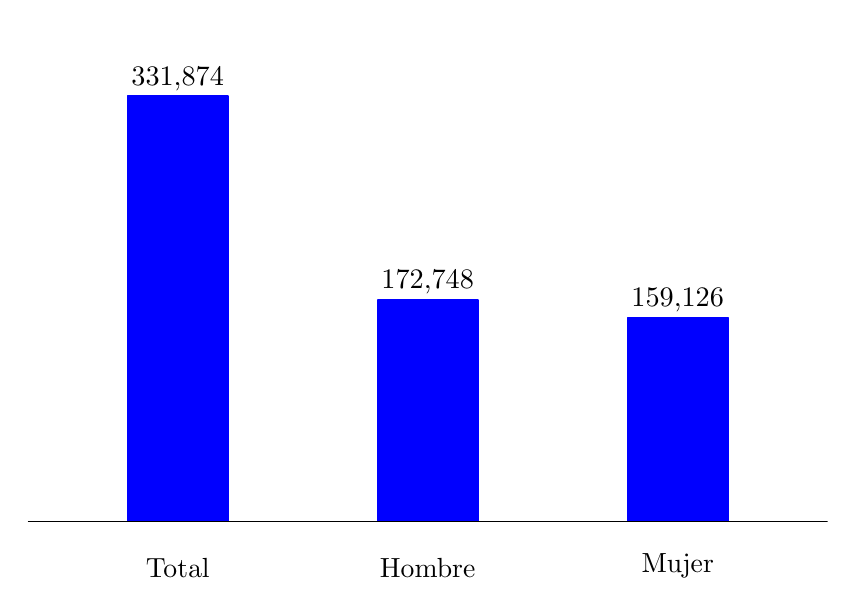
\begin{tikzpicture}[x=1pt,y=1pt]  % Created by tikzDevice version 0.9 on 2016-03-03 05:26:37
% !TEX encoding = UTF-8 Unicode
\definecolor{fillColor}{RGB}{255,255,255}
\path[use as bounding box,fill=fillColor,fill opacity=0.00] (0,0) rectangle (289.08,198.74);
\begin{scope}
\path[clip] (  0.00,  0.00) rectangle (289.08,198.74);

\path[] (  0.00,  0.00) rectangle (289.08,198.74);
\end{scope}
\begin{scope}
\path[clip] (  0.00,  0.00) rectangle (289.08,198.74);

\path[] (  0.00, 12.77) rectangle (289.08,181.67);

\path[] ( 54.20, 12.77) --
	( 54.20,181.67);

\path[] (144.54, 12.77) --
	(144.54,181.67);

\path[] (234.88, 12.77) --
	(234.88,181.67);
\definecolor{drawColor}{RGB}{0,0,255}
\definecolor{fillColor}{RGB}{0,0,255}

\path[draw=drawColor,line width= 0.6pt,line join=round,fill=fillColor] ( 36.13, 20.44) rectangle ( 72.27,173.99);

\path[draw=drawColor,line width= 0.6pt,line join=round,fill=fillColor] (126.47, 20.44) rectangle (162.61,100.37);

\path[draw=drawColor,line width= 0.6pt,line join=round,fill=fillColor] (216.81, 20.44) rectangle (252.95, 94.07);
\definecolor{drawColor}{RGB}{0,0,0}

\path[draw=drawColor,line width= 0.1pt,line join=round] (  0.00, 20.44) -- (289.08, 20.44);

\node[text=drawColor,anchor=base,inner sep=0pt, outer sep=0pt, scale=  1.02] at ( 54.20,177.96) {331,874};

\node[text=drawColor,anchor=base,inner sep=0pt, outer sep=0pt, scale=  1.02] at (144.54,104.34) {172,748};

\node[text=drawColor,anchor=base,inner sep=0pt, outer sep=0pt, scale=  1.02] at (234.88, 98.04) {159,126};

\path[] (  0.00, 12.77) rectangle (289.08,181.67);
\end{scope}
\begin{scope}
\path[clip] (  0.00,  0.00) rectangle (289.08,198.74);

\path[] (  0.00, 12.77) --
	(289.08, 12.77);
\end{scope}
\begin{scope}
\path[clip] (  0.00,  0.00) rectangle (289.08,198.74);

\path[] ( 54.20, 10.02) --
	( 54.20, 12.77);

\path[] (144.54, 10.02) --
	(144.54, 12.77);

\path[] (234.88, 10.02) --
	(234.88, 12.77);
\end{scope}
\begin{scope}
\path[clip] (  0.00,  0.00) rectangle (289.08,198.74);
\definecolor{drawColor}{RGB}{0,0,0}

\node[text=drawColor,anchor=base,inner sep=0pt, outer sep=0pt, scale=  1.00] at ( 54.20, -0.00) {Total};

\node[text=drawColor,anchor=base,inner sep=0pt, outer sep=0pt, scale=  1.00] at (144.54, -0.00) {Hombre };

\node[text=drawColor,anchor=base,inner sep=0pt, outer sep=0pt, scale=  1.00] at (234.88, 2.00) {Mujer};
\end{scope}
  \end{tikzpicture}}%
{%
	Sigsa} %


%#########################14########################

\cajota{%
	Casos de diarrea por departamento}%
{%
	Los departamentos que presentaron más casos de atención por diarrea fueron Huehuetenango (35,154 casos), San Marcos (34,588 casos), y Quiché (34,192 casos), mientras que los que tuvieron menos casos de atención médica por diarrea fueron Sacatepéquez (5,528 casos), Zacapa (5,468 casos), y El Progreso (4,055 casos). 
}%
{%
	Niños menores de cinco años que recibieron atención médica por diarrea por departamento} %
{%
	República de Guatemala, departamental, número de niños} %
{%
	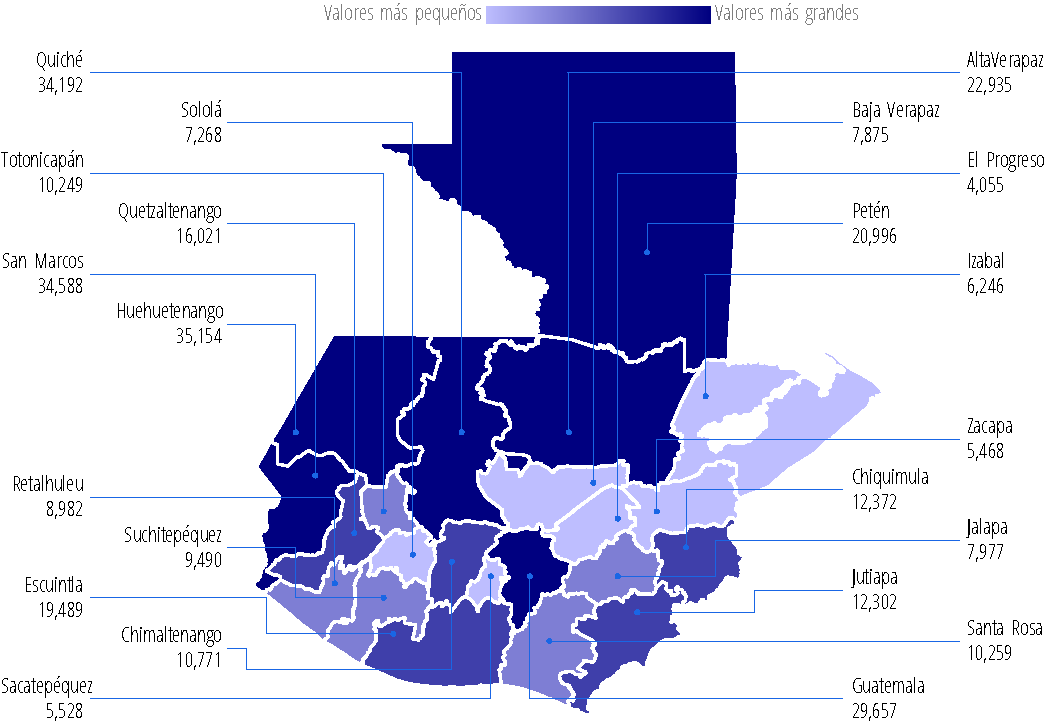
\includegraphics[width=52\cuadri]{graficas/5_14.pdf}}%
{%
	Sigsa} %


%#########################15########################

\cajita{%
	Infecciones Respiratorias Agudas (IRA)}%
{%
	En el período de 2011  a 2015 la menor cantidad de infecciones respiratorias agudas que fueron atendidas por personal médico se registró en 2015, siendo un total de 1,184,756.
}%
{%
	Niños menores de cinco años que recibieron atención médica por infecciones respiratorias agudas} %
{%
	República de Guatemala, serie histórica, número de niños} %
{%
	\begin{tikzpicture}[x=1pt,y=1pt]  \input{graficas/5_15.tex}  \end{tikzpicture}}%
{%
	Sigsa} %

%#########################16########################

\cajita{%
	Infecciones respiratorias agudas según sexo}%
{%
	Al igual que en el caso de la atención por diarreas, la cantidad de casos de IRA atendidos por personal médico es muy similar entre hombres y mujeres. 
}%
{%
	Niños menores de cinco años que recibieron atención médica por infecciones respiratorias agudas, según sexo} %
{%
	República de Guatemala, 2015, número de niños} %
{%
	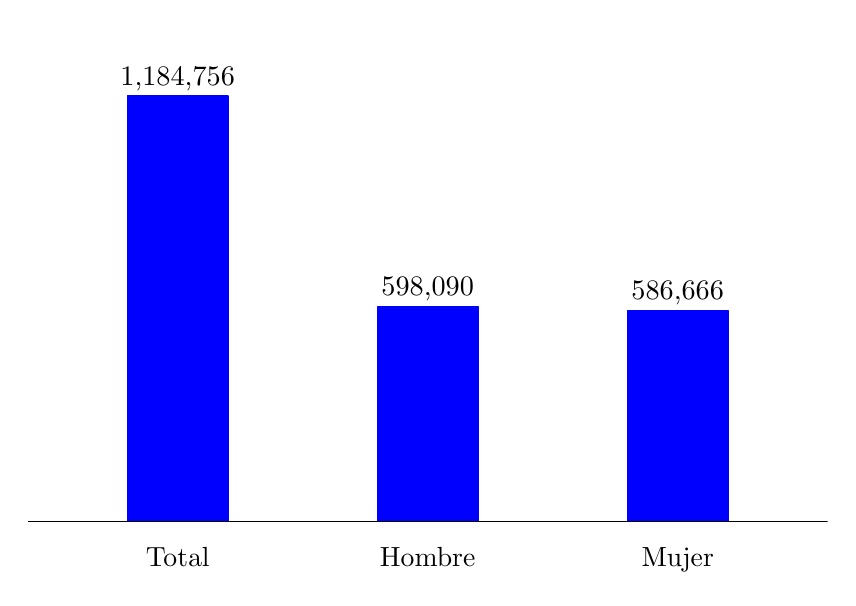
\begin{tikzpicture}[x=1pt,y=1pt]  % Created by tikzDevice version 0.9 on 2016-03-03 05:26:47
% !TEX encoding = UTF-8 Unicode
\definecolor{fillColor}{RGB}{255,255,255}
\path[use as bounding box,fill=fillColor,fill opacity=0.00] (0,0) rectangle (289.08,198.74);
\begin{scope}
\path[clip] (  0.00,  0.00) rectangle (289.08,198.74);

\path[] (  0.00,  0.00) rectangle (289.08,198.74);
\end{scope}
\begin{scope}
\path[clip] (  0.00,  0.00) rectangle (289.08,198.74);

\path[] (  0.00, 12.77) rectangle (289.08,181.67);

\path[] ( 54.20, 12.77) --
	( 54.20,181.67);

\path[] (144.54, 12.77) --
	(144.54,181.67);

\path[] (234.88, 12.77) --
	(234.88,181.67);
\definecolor{drawColor}{RGB}{0,0,255}
\definecolor{fillColor}{RGB}{0,0,255}

\path[draw=drawColor,line width= 0.6pt,line join=round,fill=fillColor] ( 36.13, 20.44) rectangle ( 72.27,173.99);

\path[draw=drawColor,line width= 0.6pt,line join=round,fill=fillColor] (126.47, 20.44) rectangle (162.61, 97.96);

\path[draw=drawColor,line width= 0.6pt,line join=round,fill=fillColor] (216.81, 20.44) rectangle (252.95, 96.48);
\definecolor{drawColor}{RGB}{0,0,0}

\path[draw=drawColor,line width= 0.1pt,line join=round] (  0.00, 20.44) -- (289.08, 20.44);

\node[text=drawColor,anchor=base,inner sep=0pt, outer sep=0pt, scale=  1.02] at ( 54.20,177.96) {1,184,756};

\node[text=drawColor,anchor=base,inner sep=0pt, outer sep=0pt, scale=  1.02] at (144.54,101.93) {598,090};

\node[text=drawColor,anchor=base,inner sep=0pt, outer sep=0pt, scale=  1.02] at (234.88,100.45) {586,666};

\path[] (  0.00, 12.77) rectangle (289.08,181.67);
\end{scope}
\begin{scope}
\path[clip] (  0.00,  0.00) rectangle (289.08,198.74);

\path[] (  0.00, 12.77) --
	(289.08, 12.77);
\end{scope}
\begin{scope}
\path[clip] (  0.00,  0.00) rectangle (289.08,198.74);

\path[] ( 54.20, 10.02) --
	( 54.20, 12.77);

\path[] (144.54, 10.02) --
	(144.54, 12.77);

\path[] (234.88, 10.02) --
	(234.88, 12.77);
\end{scope}
\begin{scope}
\path[clip] (  0.00,  0.00) rectangle (289.08,198.74);
\definecolor{drawColor}{RGB}{0,0,0}

\node[text=drawColor,anchor=base,inner sep=0pt, outer sep=0pt, scale=  1.00] at ( 54.20, 4.00) {Total};

\node[text=drawColor,anchor=base,inner sep=0pt, outer sep=0pt, scale=  1.00] at (144.54, 4.00) {Hombre};

\node[text=drawColor,anchor=base,inner sep=0pt, outer sep=0pt, scale=  1.00] at (234.88, 4.00) {Mujer};
\end{scope}
  \end{tikzpicture}}%
{%
	Sigsa} %

%#########################17########################

\cajota{%
	Casos de IRA por departamento}%
{%
	Los departamentos que registraron mayor cantidad de atención médica de casos de IRA fueron Guatemala (124,186), San Marcos (108,781) y Petén (98,928). 	Los departamentos con la menor cantidad de registros médicos de atención a casos de IRA fueron Zacapa (21,997), Sacatepéquez (20,614) y El Progreso (15,350). 
}%
{%
	Niños menores de cinco años que recibieron atención médica por infecciones respiratorias agudas por departamento} %
{%
	República de Guatemala, departamental, número de niños} %
{%
	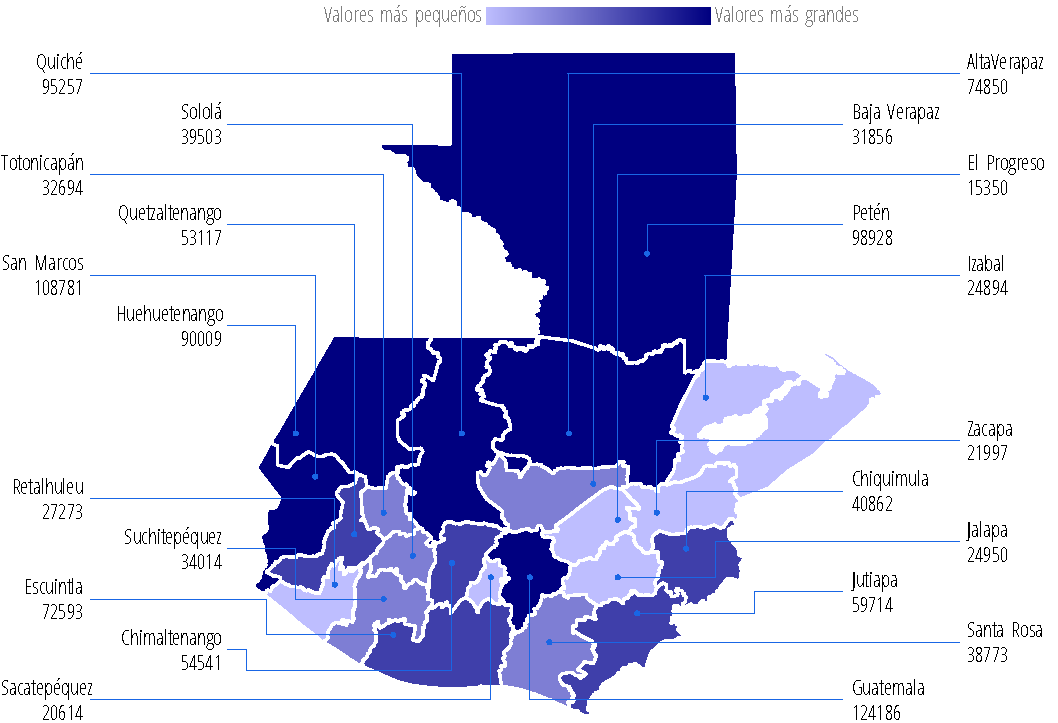
\includegraphics[width=52\cuadri]{graficas/5_17.pdf}}%
{%
	Sigsa} %



%#########################9########################
\stepcounter{section}
\begin{center}
\textbf{\color{color2}\LARGE \thesection} \quad  \textbf{\LARGE Acceso a servicios de Salud} \addcontentsline{toc}{section}{\numberline{\thesection} Acceso a servicios de Salud}
\end{center}
$ \ $ \\[-5cm]
\cajita{%
	Asistencia prenatal}%
{%

En todos los grupos de edad, el porcentaje de mujeres que recibieron atención médica prenatal de un proveedor calificado es al menos del 90\%. 
}%
{%
	Mujeres que recibieron atención prenatal de un proveedor calificado, según grupos de edad} %
{%
	República de Guatemala, 2014, en porcentaje} %
{%
	\begin{tikzpicture}[x=1pt,y=1pt]  \input{graficas/5_09.tex}  \end{tikzpicture}}%
{%
	Ensmi, 2014} %

%#########################10########################

\cajita{%
	Asistencia en el parto}%
{%
	Siete de cada diez mujeres menores de 34 años reciben algún tipo de asistencia médica a la hora del parto, mientras que para mujeres mayores de 34 años este indicador baja a seis de cada diez. 
}%
{%
	Mujeres que recibieron atención a la hora del parto  de un proveedor calificado, según grupos de edad} %
{%
	República de Guatemala, 2014, en porcentaje} %
{%
	\begin{tikzpicture}[x=1pt,y=1pt]  \input{graficas/5_10.tex}  \end{tikzpicture}}%
{%
	Ensmi, 2014} %



%#########################11########################

\cajita{%
	Niños que reciben alguna vacuna o desparasitante}%
{%
	El número de niños que recibe alguna vacuna o desparasitante aumentó en 2015 respecto al 2011. 
	
	El año que presentó mayor cantidad de niños desparasitados o vacunados fue  2012.
}%
{%
	Niños que reciben vacunas o desparasitantes} %
{%
	República de Guatemala, serie histórica, número de niños} %
{%
	\begin{tikzpicture}[x=1pt,y=1pt]  \input{graficas/5_11.tex}  \end{tikzpicture}}%
{%
	Sigsa} %

%#########################7########################

\cajita{%
	Tasa Global de Fecundidad (TGF)}%
{%	
	La Tasa Global de Fecundidad (TGF) ha ido en descenso, ya que en 1995 se ubicó en 5.1, mientras que para el 2014 llegó a 3.1 niños por mujer. 
}%
{%
	Evolución de la tasa global de fecundidad} %
{%
	República de Guatemala, serie histórica, niños por mujer} %
{%
	\begin{tikzpicture}[x=1pt,y=1pt]  \input{graficas/5_07.tex}  \end{tikzpicture}}%
{%
	Ensmi, 2014, 2008, 2002 y 1995} %

%#########################8########################

\cajita{%
	Tasa Global de Fecundidad, por área de residencia}%
{%
	Al analizar la Tasa Global de Fecundidad por área de residencia, se observa que las mujeres en el área urbana tienen menos hijos que las del área rural, esto es 2.5 contra 3.7 niños por mujer respectivamente. 
}%
{%
	Tasa global de fecundidad por área de residencia} %
{%
	República de Guatemala, 2014, niños por mujer} %
{%
	\begin{tikzpicture}[x=1pt,y=1pt]  \input{graficas/5_08.tex}  \end{tikzpicture}}%
{%
	Ensmi, 2014} %




%%%%%%%%%%%%%%%%%%%%%%%%%%%%%%%%%%13%%%%%%%%%%%%%%%%%%%%%%%%
\newpage
\stepcounter{section}
\begin{center}
\textbf{\color{color2}\LARGE \thesection} \quad  \textbf{\LARGE Acceso a servicios básicos} \addcontentsline{toc}{section}{\numberline{\thesection} Acceso a servicios básicos}
\end{center}
$\ $ \\[-2.3cm]
\cajota{%
	Acceso a agua}%
{%
	
	Para el 2011, los departamentos en los cuales más del 50\% de los hogares rurales no contaban con la disponibilidad de agua potable fueron Alta Verapaz y Retalhuleu.}%
{%
	Proporción de hogares del área rural que no poseían acceso a agua potable
} %
{%
	Por departamento, año 2011, en porcentaje} %
{%
	\includegraphics[width=52\cuadri]{graficas/1_14.pdf}}%
{%
	Instituto Nacional de Estadística (INE), Censos Municipales 2008 - 2011.} %




%%%%%%%%%%%%%%%%%%%%%%%%%%%%%%%%%%14%%%%%%%%%%%%%%%%%%%%%%%%

\cajota{%
	Acceso a servicios de saneamiento}%
{%
	Esta necesidad básica clasificada en el acceso a servicios sanitarios, toma las variables de la Encuesta Nacional de Condiciones de Vida (ENCOVI), la cual  recoge datos sobre la disponibilidad de servicios sanitarios y sistemas de eliminación de excretas.
	
	Para el 2011, el 40.4\% de los hogares rurales en Chiquimula no contaba con acceso a servicios de saneamiento, y en Jutiapa, Petén y Jalapa, tres de cada diez hogares del área rural también carecían de este servicio.   }%
{%
	Proporción de hogares del área rural sin acceso a servicios de saneamiento }
{%
	Por departamento, año 2011, en porcentaje} %
{%
	\includegraphics[width=52\cuadri]{graficas/1_15.pdf}}%
{%
	Instituto Nacional de Estadística (INE), Censos Municipales 2008 - 2011. } %


%#########################5########################
\stepcounter{section}
\begin{center}
\textbf{\color{color2}\LARGE \thesection} \quad  \textbf{\LARGE Vivienda} \addcontentsline{toc}{section}{\numberline{\thesection} Vivienda}
\end{center}
$\ $ \\[-5cm]
\cajita{%
	Viviendas y acceso al agua}%
{%
	Para el 2014, el 78.1\% de los hogares contaba con acceso a agua. A pesar de esto se presentan diferencias significativas entre el área rural y el área urbana, teniendo menor acceso esta última.
}%
{%
	Viviendas que tienen acceso a agua, según área de residencia} %
{%
	República de Guatemala, 2014, en porcentaje} %
{%
	\begin{tikzpicture}[x=1pt,y=1pt]  \input{graficas/5_05.tex}  \end{tikzpicture}}%
{%
	Encovi, 2014} %
	

%#########################6########################

\cajita{%
	Viviendas y acceso a drenajes}%
{%
	
	Para el 2014 en la República de Guatemala, el acceso a drenajes no alcanzaba el 50\%. Además, en el área rural apenas el 11.6\% cuenta con drenajes. 
	
}%
{%
	Viviendas que tienen acceso a drenajes según, área	 de residencia} %
{%
	República de Guatemala, 2014, en porcentaje} %
{%
	\begin{tikzpicture}[x=1pt,y=1pt]  \input{graficas/5_06.tex}  \end{tikzpicture}}%
{%
	Encovi, 2014} %



%#########################1########################

 \cajita{%
Viviendas formales }%
{%
	En la República, el 91.4\% de los hogares que no son pobres tiene una vivienda formal, mientras que cerca del 20\%  de los hogares que está en pobreza extrema no cuenta con una vivienda formal.  
 }%
{%
 Hogares con viviendas formales, según tipo de pobreza} %
{%
 República de Guatemala, 2014, en porcentaje} %
{%
 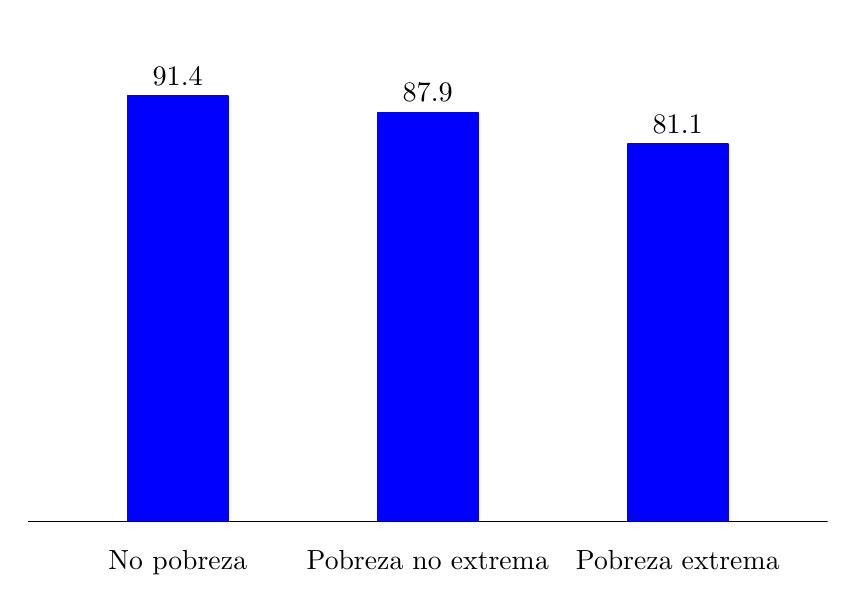
\begin{tikzpicture}[x=1pt,y=1pt]  % Created by tikzDevice version 0.9 on 2016-03-14 17:55:53
% !TEX encoding = UTF-8 Unicode
\definecolor{fillColor}{RGB}{255,255,255}
\path[use as bounding box,fill=fillColor,fill opacity=0.00] (0,0) rectangle (289.08,198.74);
\begin{scope}
\path[clip] (  0.00,  0.00) rectangle (289.08,198.74);

\path[] (  0.00,  0.00) rectangle (289.08,198.74);
\end{scope}
\begin{scope}
\path[clip] (  0.00,  0.00) rectangle (289.08,198.74);

\path[] (  0.00, 12.77) rectangle (289.08,181.67);

\path[] ( 54.20, 12.77) --
	( 54.20,181.67);

\path[] (144.54, 12.77) --
	(144.54,181.67);

\path[] (234.88, 12.77) --
	(234.88,181.67);
\definecolor{drawColor}{RGB}{0,0,255}
\definecolor{fillColor}{RGB}{0,0,255}

\path[draw=drawColor,line width= 0.6pt,line join=round,fill=fillColor] ( 36.13, 20.44) rectangle ( 72.27,173.99);

\path[draw=drawColor,line width= 0.6pt,line join=round,fill=fillColor] (126.47, 20.44) rectangle (162.61,168.11);

\path[draw=drawColor,line width= 0.6pt,line join=round,fill=fillColor] (216.81, 20.44) rectangle (252.95,156.69);
\definecolor{drawColor}{RGB}{0,0,0}

\path[draw=drawColor,line width= 0.1pt,line join=round] (  0.00, 20.44) -- (289.08, 20.44);

\node[text=drawColor,anchor=base,inner sep=0pt, outer sep=0pt, scale=  1.02] at ( 54.20,177.96) {91.4};

\node[text=drawColor,anchor=base,inner sep=0pt, outer sep=0pt, scale=  1.02] at (144.54,172.08) {87.9};

\node[text=drawColor,anchor=base,inner sep=0pt, outer sep=0pt, scale=  1.02] at (234.88,160.66) {81.1};

\path[] (  0.00, 12.77) rectangle (289.08,181.67);
\end{scope}
\begin{scope}
\path[clip] (  0.00,  0.00) rectangle (289.08,198.74);

\path[] (  0.00, 12.77) --
	(289.08, 12.77);
\end{scope}
\begin{scope}
\path[clip] (  0.00,  0.00) rectangle (289.08,198.74);

\path[] ( 54.20, 10.02) --
	( 54.20, 12.77);

\path[] (144.54, 10.02) --
	(144.54, 12.77);

\path[] (234.88, 10.02) --
	(234.88, 12.77);
\end{scope}
\begin{scope}
\path[clip] (  0.00,  0.00) rectangle (289.08,198.74);
\definecolor{drawColor}{RGB}{0,0,0}

\node[text=drawColor,anchor=base,inner sep=0pt, outer sep=0pt, scale=  1.00] at ( 54.20, 3.00) {No pobreza};

\node[text=drawColor,anchor=base,inner sep=0pt, outer sep=0pt, scale=  1.00] at (144.54, 3.00) {Pobreza no extrema};

\node[text=drawColor,anchor=base,inner sep=0pt, outer sep=0pt, scale=  1.00] at (234.88, 3.00) {Pobreza extrema};
\end{scope}
  \end{tikzpicture}}%
{%
 Encovi, 2014} %



%%%%%%%%%%%%%%%%%%%%%%%%%%%%%%%%%%12%%%%%%%%%%%%%%%%%%%%%%%%

\cajota{%
	Hogares que viven en hacinamiento en los departamentos}%
{% 
	El hacinamiento toma las variables de la Encuesta Nacional de Condiciones de Vida (ENCOVI), las cuales  recogen información sobre el número de personas en el hogar y el número de cuartos de la vivienda. 	Los departamentos con mayor porcentaje de hogares en el área rural que vivían en hacinamiento en el 2011 fueron: Alta Verapaz (64.8\%), Quiché (59.9\%), Huehuetenango (54.6\%), San Marcos (54.6\%), Suchitepéquez (52.7\%), Izabal (52.5\%), Petén (51.4\%), y Jalapa (51.4\%). }%
{%
	Proporción de hogares del área rural que vive en hacinamiento
} %
{%
	Por departamento, año 2011, en porcentaje} %
{%
	\includegraphics[width=52\cuadri]{graficas/1_13.pdf}}%
{%
 Encovi, 2014} %


%#########################2########################

\cajita{%
	Viviendas con pared de block }%
{%
	Para el 2014, apenas el 22\% de los hogares en pobreza extrema tenía una vivienda con pared de block, mientras que en los hogares que  no son pobres este indicador se ubicaba en 75.7\%. 
}%
{%
	Viviendas con pared de block, según tipo de pobreza} %
{%
	República de Guatemala, 2014, en porcentaje} %
{%
	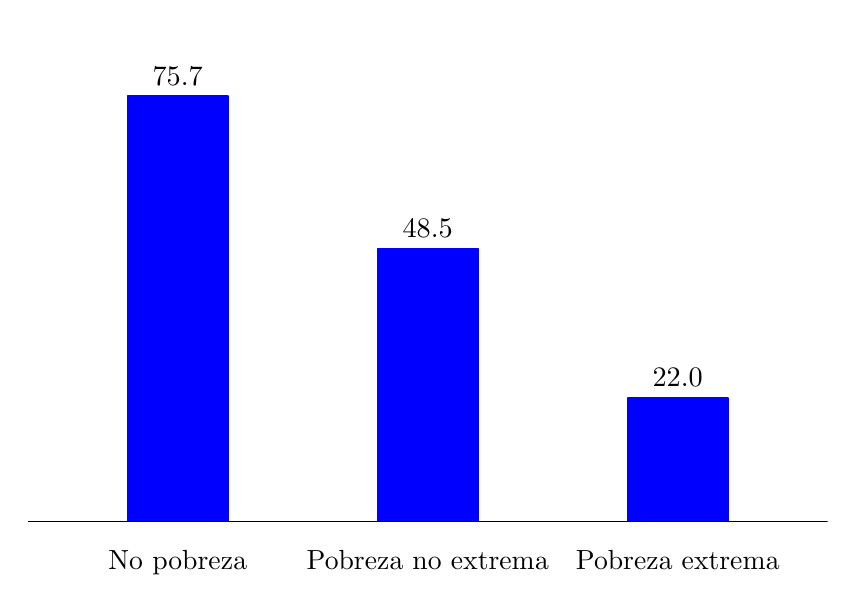
\begin{tikzpicture}[x=1pt,y=1pt]  % Created by tikzDevice version 0.9 on 2016-03-14 17:57:53
% !TEX encoding = UTF-8 Unicode
\definecolor{fillColor}{RGB}{255,255,255}
\path[use as bounding box,fill=fillColor,fill opacity=0.00] (0,0) rectangle (289.08,198.74);
\begin{scope}
\path[clip] (  0.00,  0.00) rectangle (289.08,198.74);

\path[] (  0.00,  0.00) rectangle (289.08,198.74);
\end{scope}
\begin{scope}
\path[clip] (  0.00,  0.00) rectangle (289.08,198.74);

\path[] (  0.00, 12.77) rectangle (289.08,181.67);

\path[] ( 54.20, 12.77) --
	( 54.20,181.67);

\path[] (144.54, 12.77) --
	(144.54,181.67);

\path[] (234.88, 12.77) --
	(234.88,181.67);
\definecolor{drawColor}{RGB}{0,0,255}
\definecolor{fillColor}{RGB}{0,0,255}

\path[draw=drawColor,line width= 0.6pt,line join=round,fill=fillColor] ( 36.13, 20.44) rectangle ( 72.27,173.99);

\path[draw=drawColor,line width= 0.6pt,line join=round,fill=fillColor] (126.47, 20.44) rectangle (162.61,118.90);

\path[draw=drawColor,line width= 0.6pt,line join=round,fill=fillColor] (216.81, 20.44) rectangle (252.95, 65.03);
\definecolor{drawColor}{RGB}{0,0,0}

\path[draw=drawColor,line width= 0.1pt,line join=round] (  0.00, 20.44) -- (289.08, 20.44);

\node[text=drawColor,anchor=base,inner sep=0pt, outer sep=0pt, scale=  1.02] at ( 54.20,177.96) {75.7};

\node[text=drawColor,anchor=base,inner sep=0pt, outer sep=0pt, scale=  1.02] at (144.54,122.87) {48.5};

\node[text=drawColor,anchor=base,inner sep=0pt, outer sep=0pt, scale=  1.02] at (234.88, 69.00) {22.0};

\path[] (  0.00, 12.77) rectangle (289.08,181.67);
\end{scope}
\begin{scope}
\path[clip] (  0.00,  0.00) rectangle (289.08,198.74);

\path[] (  0.00, 12.77) --
	(289.08, 12.77);
\end{scope}
\begin{scope}
\path[clip] (  0.00,  0.00) rectangle (289.08,198.74);

\path[] ( 54.20, 10.02) --
	( 54.20, 12.77);

\path[] (144.54, 10.02) --
	(144.54, 12.77);

\path[] (234.88, 10.02) --
	(234.88, 12.77);
\end{scope}
\begin{scope}
\path[clip] (  0.00,  0.00) rectangle (289.08,198.74);
\definecolor{drawColor}{RGB}{0,0,0}

\node[text=drawColor,anchor=base,inner sep=0pt, outer sep=0pt, scale=  1.00] at ( 54.20, 3.00) {No pobreza};

\node[text=drawColor,anchor=base,inner sep=0pt, outer sep=0pt, scale=  1.00] at (144.54, 3.00) {Pobreza no extrema};

\node[text=drawColor,anchor=base,inner sep=0pt, outer sep=0pt, scale=  1.00] at (234.88, 3.00) {Pobreza extrema};
\end{scope}
  \end{tikzpicture}}%
{%
	Encovi, 2014} %

%#########################3########################

\cajita{%
	Viviendas con techo de lámina }%
{%
Los hogares que no son pobres utilizan en menor medida la lámina para la construcción del techo, con una diferencia cercana a los 25 puntos respecto a los hogares en pobreza extrema. 
	}%
{%
	Viviendas con techo de lámina,  según tipo de pobreza} %
{%
	República de Guatemala, 2014, en porcentaje} %
{%
	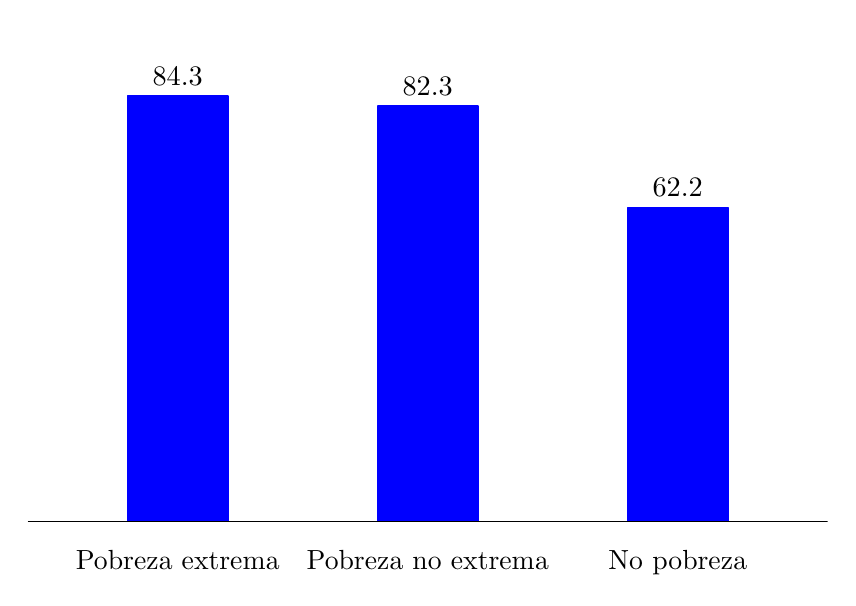
\begin{tikzpicture}[x=1pt,y=1pt]  % Created by tikzDevice version 0.9 on 2016-03-14 17:57:53
% !TEX encoding = UTF-8 Unicode
\definecolor{fillColor}{RGB}{255,255,255}
\path[use as bounding box,fill=fillColor,fill opacity=0.00] (0,0) rectangle (289.08,198.74);
\begin{scope}
\path[clip] (  0.00,  0.00) rectangle (289.08,198.74);

\path[] (  0.00,  0.00) rectangle (289.08,198.74);
\end{scope}
\begin{scope}
\path[clip] (  0.00,  0.00) rectangle (289.08,198.74);

\path[] (  0.00, 12.77) rectangle (289.08,181.67);

\path[] ( 54.20, 12.77) --
	( 54.20,181.67);

\path[] (144.54, 12.77) --
	(144.54,181.67);

\path[] (234.88, 12.77) --
	(234.88,181.67);
\definecolor{drawColor}{RGB}{0,0,255}
\definecolor{fillColor}{RGB}{0,0,255}

\path[draw=drawColor,line width= 0.6pt,line join=round,fill=fillColor] ( 36.13, 20.44) rectangle ( 72.27,173.99);

\path[draw=drawColor,line width= 0.6pt,line join=round,fill=fillColor] (126.47, 20.44) rectangle (162.61,170.40);

\path[draw=drawColor,line width= 0.6pt,line join=round,fill=fillColor] (216.81, 20.44) rectangle (252.95,133.74);
\definecolor{drawColor}{RGB}{0,0,0}

\path[draw=drawColor,line width= 0.1pt,line join=round] (  0.00, 20.44) -- (289.08, 20.44);

\node[text=drawColor,anchor=base,inner sep=0pt, outer sep=0pt, scale=  1.02] at ( 54.20,177.96) {84.3};

\node[text=drawColor,anchor=base,inner sep=0pt, outer sep=0pt, scale=  1.02] at (144.54,174.38) {82.3};

\node[text=drawColor,anchor=base,inner sep=0pt, outer sep=0pt, scale=  1.02] at (234.88,137.71) {62.2};

\path[] (  0.00, 12.77) rectangle (289.08,181.67);
\end{scope}
\begin{scope}
\path[clip] (  0.00,  0.00) rectangle (289.08,198.74);

\path[] (  0.00, 12.77) --
	(289.08, 12.77);
\end{scope}
\begin{scope}
\path[clip] (  0.00,  0.00) rectangle (289.08,198.74);

\path[] ( 54.20, 10.02) --
	( 54.20, 12.77);

\path[] (144.54, 10.02) --
	(144.54, 12.77);

\path[] (234.88, 10.02) --
	(234.88, 12.77);
\end{scope}
\begin{scope}
\path[clip] (  0.00,  0.00) rectangle (289.08,198.74);
\definecolor{drawColor}{RGB}{0,0,0}

\node[text=drawColor,anchor=base,inner sep=0pt, outer sep=0pt, scale=  1.00] at ( 54.20, 3.00) {Pobreza extrema};

\node[text=drawColor,anchor=base,inner sep=0pt, outer sep=0pt, scale=  1.00] at (144.54, 3.00) {Pobreza no extrema};

\node[text=drawColor,anchor=base,inner sep=0pt, outer sep=0pt, scale=  1.00] at (234.88, 3.00) {No pobreza};
\end{scope}
  \end{tikzpicture}}%
{%
	Encovi, 2014} %

%#########################4########################

\cajita{%
	Viviendas y material del piso}%
{%
	Los hogares en   pobreza extrema son los que presentan una menor proporción en el uso de torta de cemento (25.3\% contra un 67\%). Para los hogares que no son pobres predomina el uso de torta de cemento, ya que el 40.2\% de los hogares lo usa, contra un 10.4\% que usa piso de tierra. 
}%
{%
	Viviendas según material del piso y tipo de pobreza} %
{%
	República de Guatemala, 2014, en porcentaje} %
{%
	\begin{tikzpicture}[x=1pt,y=1pt]  % Created by tikzDevice version 0.9 on 2016-03-03 05:25:52
% !TEX encoding = UTF-8 Unicode
\definecolor{fillColor}{RGB}{255,255,255}
\path[use as bounding box,fill=fillColor,fill opacity=0.00] (0,0) rectangle (289.08,198.74);
\begin{scope}
\path[clip] (  0.00,  0.00) rectangle (289.08,198.74);

\path[] (  0.00,  0.00) rectangle (289.08,198.74);
\end{scope}
\begin{scope}
\path[clip] (  0.00,  0.00) rectangle (289.08,198.74);

\path[] (  0.00, 18.46) rectangle (289.08,166.57);

\path[] ( 54.20, 18.46) --
	( 54.20,166.57);

\path[] (144.54, 18.46) --
	(144.54,166.57);

\path[] (234.88, 18.46) --
	(234.88,166.57);
\definecolor{drawColor}{RGB}{0,0,255}
\definecolor{fillColor}{RGB}{0,0,255}

\path[draw=drawColor,line width= 0.6pt,line join=round,fill=fillColor] ( 15.81, 18.46) rectangle ( 51.94, 74.33);
\definecolor{drawColor}{RGB}{157,187,255}
\definecolor{fillColor}{RGB}{157,187,255}

\path[draw=drawColor,line width= 0.6pt,line join=round,fill=fillColor] ( 56.46, 18.46) rectangle ( 92.60,166.57);
\definecolor{drawColor}{RGB}{0,0,255}
\definecolor{fillColor}{RGB}{0,0,255}

\path[draw=drawColor,line width= 0.6pt,line join=round,fill=fillColor] (106.15, 18.46) rectangle (142.28,120.72);
\definecolor{drawColor}{RGB}{157,187,255}
\definecolor{fillColor}{RGB}{157,187,255}

\path[draw=drawColor,line width= 0.6pt,line join=round,fill=fillColor] (146.80, 18.46) rectangle (182.93, 95.86);
\definecolor{drawColor}{RGB}{0,0,255}
\definecolor{fillColor}{RGB}{0,0,255}

\path[draw=drawColor,line width= 0.6pt,line join=round,fill=fillColor] (196.48, 18.46) rectangle (232.62,107.27);
\definecolor{drawColor}{RGB}{157,187,255}
\definecolor{fillColor}{RGB}{157,187,255}

\path[draw=drawColor,line width= 0.6pt,line join=round,fill=fillColor] (237.14, 18.46) rectangle (273.27, 41.36);
\definecolor{drawColor}{RGB}{0,0,0}

\path[draw=drawColor,line width= 0.6pt,line join=round] (  0.00, 18.46) -- (289.08, 18.46);

\node[text=drawColor,rotate= 90.00,anchor=base west,inner sep=0pt, outer sep=0pt, scale=  0.83] at ( 37.11, 76.88) {25.3};

\node[text=drawColor,rotate= 90.00,anchor=base west,inner sep=0pt, outer sep=0pt, scale=  0.83] at ( 77.76,169.12) {67.0};

\node[text=drawColor,rotate= 90.00,anchor=base west,inner sep=0pt, outer sep=0pt, scale=  0.83] at (127.45,123.26) {46.3};

\node[text=drawColor,rotate= 90.00,anchor=base west,inner sep=0pt, outer sep=0pt, scale=  0.83] at (168.10, 98.40) {35.0};

\node[text=drawColor,rotate= 90.00,anchor=base west,inner sep=0pt, outer sep=0pt, scale=  0.83] at (217.79,109.81) {40.2};

\node[text=drawColor,rotate= 90.00,anchor=base west,inner sep=0pt, outer sep=0pt, scale=  0.83] at (258.44, 43.91) {10.4};

\path[] (  0.00, 18.46) rectangle (289.08,166.57);
\end{scope}
\begin{scope}
\path[clip] (  0.00,  0.00) rectangle (289.08,198.74);

\path[] (  0.00, 18.46) --
	(289.08, 18.46);
\end{scope}
\begin{scope}
\path[clip] (  0.00,  0.00) rectangle (289.08,198.74);

\path[] ( 54.20, 15.71) --
	( 54.20, 18.46);

\path[] (144.54, 15.71) --
	(144.54, 18.46);

\path[] (234.88, 15.71) --
	(234.88, 18.46);
\end{scope}
\begin{scope}
\path[clip] (  0.00,  0.00) rectangle (289.08,198.74);
\definecolor{drawColor}{RGB}{0,0,0}

\node[text=drawColor,anchor=base,inner sep=0pt, outer sep=0pt, scale=  1.00] at ( 54.20,  5.69) {Pobreza extrema};

\node[text=drawColor,anchor=base,inner sep=0pt, outer sep=0pt, scale=  1.00] at (144.54,  5.69) {Pobreza no extrema};

\node[text=drawColor,anchor=base,inner sep=0pt, outer sep=0pt, scale=  1.00] at (234.88,  5.69) {No pobreza};
\end{scope}
\begin{scope}
\path[clip] (  0.00,  0.00) rectangle (289.08,198.74);
\coordinate (apoyo) at (41.26,191.13);
\coordinate (longitudFicticia) at (7.11,7.61);
\coordinate (longitud) at (7.11,7.11);
\coordinate (desX) at (157.45,0);
\coordinate (desY) at (0,0.25);
\definecolor[named]{ct1}{HTML}{
0000FF
}
\definecolor[named]{ct2}{HTML}{
9DBBFF
}
\definecolor[named]{ctb1}{HTML}{
0000FF
}
\definecolor[named]{ctb2}{HTML}{
9DBBFF
}
\path [fill=none] (apoyo) rectangle ($(apoyo)+(longitudFicticia)$)
node [xshift=0.3cm,inner sep=0pt, outer sep=0pt,midway,right,scale = 0.9]{Torta de cemento};
\draw [color = ctb1,fill=ct1] ( $(apoyo)  + (desY) $) rectangle ($(apoyo)+ (desY) +(longitud)$);
\path [fill=none] ($(apoyo)+(desX)$) rectangle ($(apoyo)+(desX)+(longitudFicticia)$)
node [xshift=0.3cm,inner sep=0pt, outer sep=0pt,midway,right,scale = 0.9]{Tierra};
\draw [color = ctb2 ,fill=ct2] ( $(apoyo)  + (desY) + (desX) $) rectangle ($(apoyo)+ (desY)+ (desX) +(longitud)$);
\end{scope}
  \end{tikzpicture}}%
{%
	Encovi, 2014} %


		\INEchaptercarta{Situación y atención a la desnutrición o malnutrición}{Esta dimensión se refiere a la desnutrición aguda y la atención que se la da a la misma. La desnutrición aguda, también conocida como emaciación o bajo peso para la talla, es causada por una ingesta insuficiente de alimentos y por la presencia de infecciones graves durante períodos prolongados. Por otro lado, la desnutrición crónica o de baja talla para la edad, es el retardo en el crecimiento lineal de los niños debido a una mala alimentación e infecciones agudas repetidas (Coneval, 2010). Esta dimensión está compuesta por cuatro indicadores y veinte sub-indicadores.
			
	
		}	\begin{figure}[ht]
		\begin{adjustbox}{addcode={\begin{minipage}{\width}}{\caption{%
							Indicadores y subindicadores del capítulo 6. Situación y Atención a la Desnutrición/malnutrición. 
						} \qquad \qquad \qquad \qquad\qquad \qquad\qquad \qquad\qquad    Elaborado por: Iarna-URL, 2016.\end{minipage}},rotate=90,center}
			\includegraphics[scale=.45]{MapaDesnutricion.jpeg}%
		\end{adjustbox}
	\end{figure}
		\cleardoublepage
	\stepcounter{section}
\begin{center}
	\textbf{\color{color2}\LARGE \thesection} \quad  \textbf{\LARGE Situación nutricional de la madre} \addcontentsline{toc}{section}{\numberline{\thesection} Situación nutricional de la madre}
\end{center}
$ \ $ \\[-5cm]%#########################1########################

 \cajita{%
Mujeres con anemia }%
{Para el año 2008 se registró que del total de las madres embarazadas el 29.1\% padecía anemia, mientras que en las mujeres que no se encontraban en gestación el porcentaje de anemia bajó en 7.7 puntos porcentuales. 
 }%
{%
 Mujeres con anemia, según estado de gestación} %
{%
 República de Guatemala, 2008-2009, en porcentaje} %
{%
 \begin{tikzpicture}[x=1pt,y=1pt]  \input{graficas/6_01.tex}  \end{tikzpicture}}%
{%
Encuesta Nacional de Salud Materno Infantil (Ensmi), 2008/2009 } %

%#########################2########################

\cajita{%
	Índice de Masa Corporal (IMC) de mujeres  }%
{%
	La mayoría de las mujeres guatemaltecas que no se encontraban embarazadas en el 2008 presentaba un IMC normal, mientras que solo un 1.6\% tenía IMC bajo. 
}%
{%
	Índice de masa corporal de mujeres no embarazadas} %
{%
	República de Guatemala, 2008-2009, en porcentaje} %
{%
	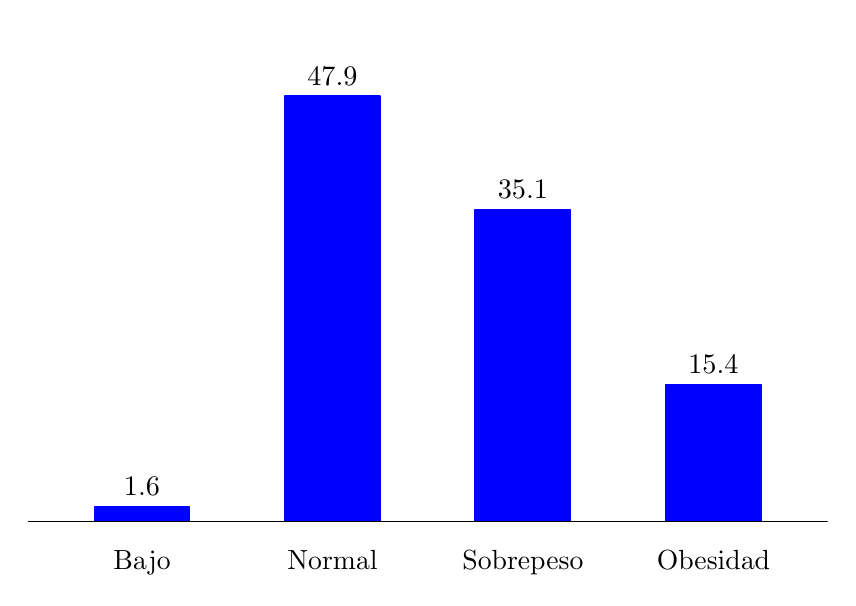
\begin{tikzpicture}[x=1pt,y=1pt]  % Created by tikzDevice version 0.9 on 2016-03-03 06:06:28
% !TEX encoding = UTF-8 Unicode
\definecolor{fillColor}{RGB}{255,255,255}
\path[use as bounding box,fill=fillColor,fill opacity=0.00] (0,0) rectangle (289.08,198.74);
\begin{scope}
\path[clip] (  0.00,  0.00) rectangle (289.08,198.74);

\path[] (  0.00,  0.00) rectangle (289.08,198.74);
\end{scope}
\begin{scope}
\path[clip] (  0.00,  0.00) rectangle (289.08,198.74);

\path[] (  0.00, 12.77) rectangle (289.08,181.67);

\path[] ( 41.30, 12.77) --
	( 41.30,181.67);

\path[] (110.13, 12.77) --
	(110.13,181.67);

\path[] (178.95, 12.77) --
	(178.95,181.67);

\path[] (247.78, 12.77) --
	(247.78,181.67);
\definecolor{drawColor}{RGB}{0,0,255}
\definecolor{fillColor}{RGB}{0,0,255}

\path[draw=drawColor,line width= 0.6pt,line join=round,fill=fillColor] ( 24.09, 20.44) rectangle ( 58.50, 25.57);

\path[draw=drawColor,line width= 0.6pt,line join=round,fill=fillColor] ( 92.92, 20.44) rectangle (127.33,173.99);

\path[draw=drawColor,line width= 0.6pt,line join=round,fill=fillColor] (161.75, 20.44) rectangle (196.16,132.96);

\path[draw=drawColor,line width= 0.6pt,line join=round,fill=fillColor] (230.58, 20.44) rectangle (264.99, 69.81);
\definecolor{drawColor}{RGB}{0,0,0}

\path[draw=drawColor,line width= 0.1pt,line join=round] (  0.00, 20.44) -- (289.08, 20.44);

\node[text=drawColor,anchor=base,inner sep=0pt, outer sep=0pt, scale=  1.02] at ( 41.30, 29.54) {1.6};

\node[text=drawColor,anchor=base,inner sep=0pt, outer sep=0pt, scale=  1.02] at (110.13,177.96) {47.9};

\node[text=drawColor,anchor=base,inner sep=0pt, outer sep=0pt, scale=  1.02] at (178.95,136.93) {35.1};

\node[text=drawColor,anchor=base,inner sep=0pt, outer sep=0pt, scale=  1.02] at (247.78, 73.78) {15.4};

\path[] (  0.00, 12.77) rectangle (289.08,181.67);
\end{scope}
\begin{scope}
\path[clip] (  0.00,  0.00) rectangle (289.08,198.74);

\path[] (  0.00, 12.77) --
	(289.08, 12.77);
\end{scope}
\begin{scope}
\path[clip] (  0.00,  0.00) rectangle (289.08,198.74);

\path[] ( 41.30, 10.02) --
	( 41.30, 12.77);

\path[] (110.13, 10.02) --
	(110.13, 12.77);

\path[] (178.95, 10.02) --
	(178.95, 12.77);

\path[] (247.78, 10.02) --
	(247.78, 12.77);
\end{scope}
\begin{scope}
\path[clip] (  0.00,  0.00) rectangle (289.08,198.74);
\definecolor{drawColor}{RGB}{0,0,0}

\node[text=drawColor,anchor=base,inner sep=0pt, outer sep=0pt, scale=  1.00] at ( 41.30, 3.00) {Bajo};

\node[text=drawColor,anchor=base,inner sep=0pt, outer sep=0pt, scale=  1.00] at (110.13, 3.00) {Normal};

\node[text=drawColor,anchor=base,inner sep=0pt, outer sep=0pt, scale=  1.00] at (178.95, 3.00) {Sobrepeso};

\node[text=drawColor,anchor=base,inner sep=0pt, outer sep=0pt, scale=  1.00] at (247.78, 3.00) {Obesidad};
\end{scope}
  \end{tikzpicture}}%
{%
	Encuesta Nacional de Salud Materno Infantil (Ensmi), 2008/2009} %


%#########################3########################

\cajita{%
	IMC de mujeres, según área de residencia }%
{%
	En el área urbana se presenta mayor proporción de mujeres con sobrepeso y obesidad (37.5\% y 20.3\%) que en el área rural (33.4\% y 12.1\%). 
	Además, el área rural presenta mayor proporción de mujeres con IMC normal que el área urbana. 
}%
{%
	Índice de Masa Corporal (IMC) de mujeres no embarazadas, según área de residencia} %
{%
	República de Guatemala, 2008-2009, en porcentaje} %
{%
	\begin{tikzpicture}[x=1pt,y=1pt]  % Created by tikzDevice version 0.9 on 2016-03-03 06:06:32
% !TEX encoding = UTF-8 Unicode
\definecolor{fillColor}{RGB}{255,255,255}
\path[use as bounding box,fill=fillColor,fill opacity=0.00] (0,0) rectangle (289.08,198.74);
\begin{scope}
\path[clip] (  0.00,  0.00) rectangle (289.08,198.74);

\path[] (  0.00,  0.00) rectangle (289.08,198.74);
\end{scope}
\begin{scope}
\path[clip] (  0.00,  0.00) rectangle (289.08,198.74);

\path[] (  0.00, 18.46) rectangle (289.08,166.57);

\path[] ( 41.30, 18.46) --
	( 41.30,166.57);

\path[] (110.13, 18.46) --
	(110.13,166.57);

\path[] (178.95, 18.46) --
	(178.95,166.57);

\path[] (247.78, 18.46) --
	(247.78,166.57);
\definecolor{drawColor}{RGB}{0,0,255}
\definecolor{fillColor}{RGB}{0,0,255}

\path[draw=drawColor,line width= 0.6pt,line join=round,fill=fillColor] ( 12.05, 18.46) rectangle ( 39.58, 23.49);
\definecolor{drawColor}{RGB}{157,187,255}
\definecolor{fillColor}{RGB}{157,187,255}

\path[draw=drawColor,line width= 0.6pt,line join=round,fill=fillColor] ( 43.02, 18.46) rectangle ( 70.55, 22.65);
\definecolor{drawColor}{RGB}{0,0,255}
\definecolor{fillColor}{RGB}{0,0,255}

\path[draw=drawColor,line width= 0.6pt,line join=round,fill=fillColor] ( 80.87, 18.46) rectangle (108.40,131.64);
\definecolor{drawColor}{RGB}{157,187,255}
\definecolor{fillColor}{RGB}{157,187,255}

\path[draw=drawColor,line width= 0.6pt,line join=round,fill=fillColor] (111.85, 18.46) rectangle (139.38,166.57);
\definecolor{drawColor}{RGB}{0,0,255}
\definecolor{fillColor}{RGB}{0,0,255}

\path[draw=drawColor,line width= 0.6pt,line join=round,fill=fillColor] (149.70, 18.46) rectangle (177.23,123.26);
\definecolor{drawColor}{RGB}{157,187,255}
\definecolor{fillColor}{RGB}{157,187,255}

\path[draw=drawColor,line width= 0.6pt,line join=round,fill=fillColor] (180.68, 18.46) rectangle (208.21,111.80);
\definecolor{drawColor}{RGB}{0,0,255}
\definecolor{fillColor}{RGB}{0,0,255}

\path[draw=drawColor,line width= 0.6pt,line join=round,fill=fillColor] (218.53, 18.46) rectangle (246.06, 75.19);
\definecolor{drawColor}{RGB}{157,187,255}
\definecolor{fillColor}{RGB}{157,187,255}

\path[draw=drawColor,line width= 0.6pt,line join=round,fill=fillColor] (249.50, 18.46) rectangle (277.03, 52.27);
\definecolor{drawColor}{RGB}{0,0,0}

\path[draw=drawColor,line width= 0.6pt,line join=round] (  0.00, 18.46) -- (289.08, 18.46);

\node[text=drawColor,anchor=base west,inner sep=0pt, outer sep=0pt, scale=  0.83] at ( 23.05, 25.31) {1.8};

\node[text=drawColor,anchor=base west,inner sep=0pt, outer sep=0pt, scale=  0.83] at ( 54.02, 24.47) {1.5};

\node[text=drawColor,anchor=base west,inner sep=0pt, outer sep=0pt, scale=  0.83] at ( 91.87,134.19) {40.5};

\node[text=drawColor,anchor=base west,inner sep=0pt, outer sep=0pt, scale=  0.83] at (122.85,169.12) {53.0};

\node[text=drawColor,anchor=base west,inner sep=0pt, outer sep=0pt, scale=  0.83] at (160.70,125.81) {37.5};

\node[text=drawColor,anchor=base west,inner sep=0pt, outer sep=0pt, scale=  0.83] at (191.68,114.35) {33.4};

\node[text=drawColor,anchor=base west,inner sep=0pt, outer sep=0pt, scale=  0.83] at (229.53, 77.74) {20.3};

\node[text=drawColor,anchor=base west,inner sep=0pt, outer sep=0pt, scale=  0.83] at (260.50, 54.82) {12.1};

\path[] (  0.00, 18.46) rectangle (289.08,166.57);
\end{scope}
\begin{scope}
\path[clip] (  0.00,  0.00) rectangle (289.08,198.74);

\path[] (  0.00, 18.46) --
	(289.08, 18.46);
\end{scope}
\begin{scope}
\path[clip] (  0.00,  0.00) rectangle (289.08,198.74);

\path[] ( 41.30, 15.71) --
	( 41.30, 18.46);

\path[] (110.13, 15.71) --
	(110.13, 18.46);

\path[] (178.95, 15.71) --
	(178.95, 18.46);

\path[] (247.78, 15.71) --
	(247.78, 18.46);
\end{scope}
\begin{scope}
\path[clip] (  0.00,  0.00) rectangle (289.08,198.74);
\definecolor{drawColor}{RGB}{0,0,0}

\node[text=drawColor,anchor=base,inner sep=0pt, outer sep=0pt, scale=  1.00] at ( 41.30,  5.69) {Bajo};

\node[text=drawColor,anchor=base,inner sep=0pt, outer sep=0pt, scale=  1.00] at (110.13,  5.69) {Normal};

\node[text=drawColor,anchor=base,inner sep=0pt, outer sep=0pt, scale=  1.00] at (178.95,  5.69) {Sobre peso};

\node[text=drawColor,anchor=base,inner sep=0pt, outer sep=0pt, scale=  1.00] at (247.78,  5.69) {Obesidad};
\end{scope}
\begin{scope}
\path[clip] (  0.00,  0.00) rectangle (289.08,198.74);
\coordinate (apoyo) at (57.27,191.13);
\coordinate (longitudFicticia) at (7.11,7.61);
\coordinate (longitud) at (7.11,7.11);
\coordinate (desX) at (142.24,0);
\coordinate (desY) at (0,0.25);
\definecolor[named]{ct1}{HTML}{
0000FF
}
\definecolor[named]{ct2}{HTML}{
9DBBFF
}
\definecolor[named]{ctb1}{HTML}{
0000FF
}
\definecolor[named]{ctb2}{HTML}{
9DBBFF
}
\path [fill=none] (apoyo) rectangle ($(apoyo)+(longitudFicticia)$)
node [xshift=0.3cm,inner sep=0pt, outer sep=0pt,midway,right,scale = 0.9]{Urbana};
\draw [color = ctb1,fill=ct1] ( $(apoyo)  + (desY) $) rectangle ($(apoyo)+ (desY) +(longitud)$);
\path [fill=none] ($(apoyo)+(desX)$) rectangle ($(apoyo)+(desX)+(longitudFicticia)$)
node [xshift=0.3cm,inner sep=0pt, outer sep=0pt,midway,right,scale = 0.9]{Rural};
\draw [color = ctb2 ,fill=ct2] ( $(apoyo)  + (desY) + (desX) $) rectangle ($(apoyo)+ (desY)+ (desX) +(longitud)$);
\end{scope}
  \end{tikzpicture}}%
{%
	Encuesta Nacional de Salud Materno Infantil (Ensmi), 2008/2009} %


%#########################4########################

\cajita{%
	Talla promedio según área de residencia }%
{%
	Para el 2008 la talla\footnote{Hace referencia a la estatura de una persona, y en este caso se presenta en centímetros.} para madres del área urbana de niños menores de 5 años es apenas mayor que la de las madres del área rural. 
}%
{%
	Talla promedio de madres  de niños menores de 5 años, según área de residencia} %
{%
	República de Guatemala, 2008-2009, en centímetros} %
{%
	\begin{tikzpicture}[x=1pt,y=1pt]  \input{graficas/6_04.tex}  \end{tikzpicture}}%
{%
	Encuesta Nacional de Salud Materno Infantil (Ensmi), 2008/2009} %

%#########################5########################
\stepcounter{section}
\begin{center}
	\textbf{\color{color2}\LARGE \thesection} \quad  \textbf{\LARGE Situación nutricional del niño} \addcontentsline{toc}{section}{\numberline{\thesection} Situación nutricional del niño}
\end{center} $ \ $\\[-5cm]
\cajita{%
	Peso de niños recién nacidos }%
{%
	Uno de los datos más importantes que debe ser medido en un neonato es el peso.
	Para el 2008, el 88.1\% de los recién nacidos presentó un peso no menor de  2.5 kilogramos. 
}%
{%
	Distribución de niños recién nacidos, según peso (en kilogramos), reportado por la madre} %
{%
	República de Guatemala, 2008-2009, en porcentaje} %
{%
	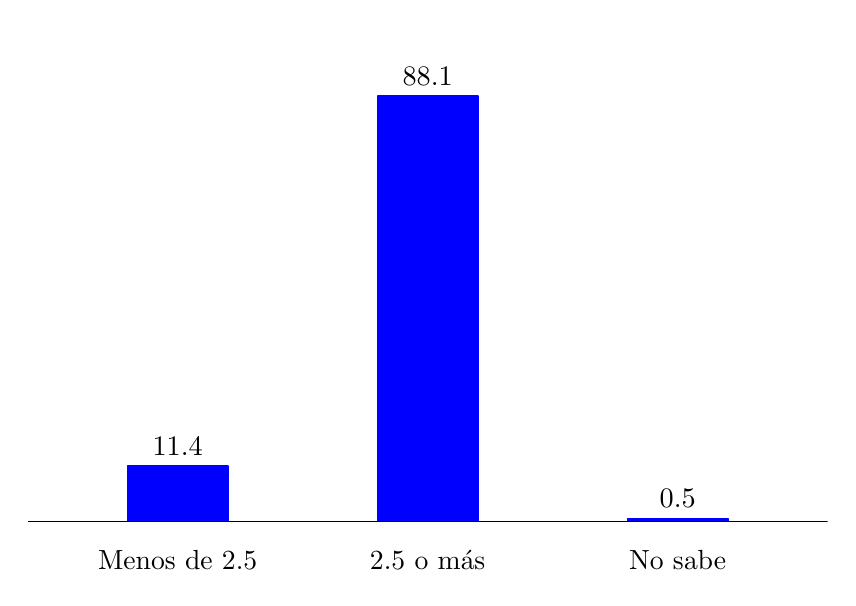
\begin{tikzpicture}[x=1pt,y=1pt]  % Created by tikzDevice version 0.9 on 2016-03-03 06:06:40
% !TEX encoding = UTF-8 Unicode
\definecolor{fillColor}{RGB}{255,255,255}
\path[use as bounding box,fill=fillColor,fill opacity=0.00] (0,0) rectangle (289.08,198.74);
\begin{scope}
\path[clip] (  0.00,  0.00) rectangle (289.08,198.74);

\path[] (  0.00,  0.00) rectangle (289.08,198.74);
\end{scope}
\begin{scope}
\path[clip] (  0.00,  0.00) rectangle (289.08,198.74);

\path[] (  0.00, 12.77) rectangle (289.08,181.67);

\path[] ( 54.20, 12.77) --
	( 54.20,181.67);

\path[] (144.54, 12.77) --
	(144.54,181.67);

\path[] (234.88, 12.77) --
	(234.88,181.67);
\definecolor{drawColor}{RGB}{0,0,255}
\definecolor{fillColor}{RGB}{0,0,255}

\path[draw=drawColor,line width= 0.6pt,line join=round,fill=fillColor] ( 36.13, 20.44) rectangle ( 72.27, 40.31);

\path[draw=drawColor,line width= 0.6pt,line join=round,fill=fillColor] (126.47, 20.44) rectangle (162.61,173.99);

\path[draw=drawColor,line width= 0.6pt,line join=round,fill=fillColor] (216.81, 20.44) rectangle (252.95, 21.32);
\definecolor{drawColor}{RGB}{0,0,0}

\path[draw=drawColor,line width= 0.1pt,line join=round] (  0.00, 20.44) -- (289.08, 20.44);

\node[text=drawColor,anchor=base,inner sep=0pt, outer sep=0pt, scale=  1.02] at ( 54.20, 44.28) {11.4};

\node[text=drawColor,anchor=base,inner sep=0pt, outer sep=0pt, scale=  1.02] at (144.54,177.96) {88.1};

\node[text=drawColor,anchor=base,inner sep=0pt, outer sep=0pt, scale=  1.02] at (234.88, 25.29) {0.5};

\path[] (  0.00, 12.77) rectangle (289.08,181.67);
\end{scope}
\begin{scope}
\path[clip] (  0.00,  0.00) rectangle (289.08,198.74);

\path[] (  0.00, 12.77) --
	(289.08, 12.77);
\end{scope}
\begin{scope}
\path[clip] (  0.00,  0.00) rectangle (289.08,198.74);

\path[] ( 54.20, 10.02) --
	( 54.20, 12.77);

\path[] (144.54, 10.02) --
	(144.54, 12.77);

\path[] (234.88, 10.02) --
	(234.88, 12.77);
\end{scope}
\begin{scope}
\path[clip] (  0.00,  0.00) rectangle (289.08,198.74);
\definecolor{drawColor}{RGB}{0,0,0}

\node[text=drawColor,anchor=base,inner sep=0pt, outer sep=0pt, scale=  1.00] at ( 54.20, 3.00) {Menos de 2.5 };

\node[text=drawColor,anchor=base,inner sep=0pt, outer sep=0pt, scale=  1.00] at (144.54, 3.00) {2.5  o más};

\node[text=drawColor,anchor=base,inner sep=0pt, outer sep=0pt, scale=  1.00] at (234.88, 3.00) {No sabe};
\end{scope}
  \end{tikzpicture}}%
{%
	Encuesta Nacional de Salud Materno Infantil (Ensmi), 2008/2009} %

%#########################6########################

\cajita{%
	Desnutrición global }%
{%
	La tasa de desnutricion global total para el 2008 fue de 13.1\%, siendo el 2.1\% desnutrición global severa. 
}%
{%
	Niños menores de 5 años con desnutrición global} %
{%
	República de Guatemala, 2008-2009, en porcentaje} %
{%
	\begin{tikzpicture}[x=1pt,y=1pt]  \input{graficas/6_05.tex}  \end{tikzpicture}}%
{%
	Encuesta Nacional de Salud Materno Infantil (Ensmi), 2008/2009} %

%#########################7########################

\cajita{%
	Desnutrición aguda }%
{%
	La desnutrición aguda (bajo peso para la talla) se ubicó en 1.4\% para el 2008.
}%
{%
	Niños menores de 5 años con desnutrición aguda} %
{%
	República de Guatemala, 2008-2009, en porcentaje} %
{%
	\begin{tikzpicture}[x=1pt,y=1pt]  \input{graficas/6_06.tex}  \end{tikzpicture}}%
{%
	Encuesta Nacional de Salud Materno Infantil (Ensmi), 2008/2009} %


%#########################8########################

\cajita{%
	Desnutrición crónica }%
{%
	La desnutrición crónica es el retraso del crecimiento esperado para una edad. 
	
	Para niños menores de 5 años se observó en 2008 que el 49.8\% de estos presenta una talla menor a la esperada para su edad, es decir que se encontraban con desnutrición crónica. 
}%
{%
	Niños menores de 5 años con desnutrición crónica} %
{%
	República de Guatemala, 2008-2009, en porcentaje} %
{%
	\begin{tikzpicture}[x=1pt,y=1pt]  \input{graficas/6_07.tex}  \end{tikzpicture}}%
{%
	Encuesta Nacional de Salud Materno Infantil (Ensmi), 2008/2009} %


%#########################9########################

\cajita{%
	Niños con anemia }%
{%
	El área rural presenta mayor porcentaje de niños con anemia, ubicándose en 48.6\%, esto está 2.4 puntos por arriba del indicador para el área urbana. 
	}%
{%
	Niños entre 6 y 59 meses con anemia, según área de residencia} %
{%
	República de Guatemala, 2008-2009, en porcentaje} %
{%
	\begin{tikzpicture}[x=1pt,y=1pt]  \input{graficas/6_08.tex}  \end{tikzpicture}}%
{%
	Encuesta Nacional de Salud Materno Infantil (Ensmi), 2008/2009} %

%#########################9########################

\cajota{%
	Niños con anemia por departamento }%
{%
	El departamento de Suchitepéquez es el que presenta menor porcentaje de niños con anemia (37.7\%), seguido de El Progreso (37.8\%), y Quetzaltenango (40.2\%). Los departamentos con mayor porcentaje de anemia en niños son Totonicapán (62.2\%), Sololá (56.1\%), y Chiquimula (55.5\%).
}%
{%
	Niños entre 6 y 59 meses con anemia por departamento} %
{%
	República de Guatemala, 2008-2009, en porcentaje} %
{%
	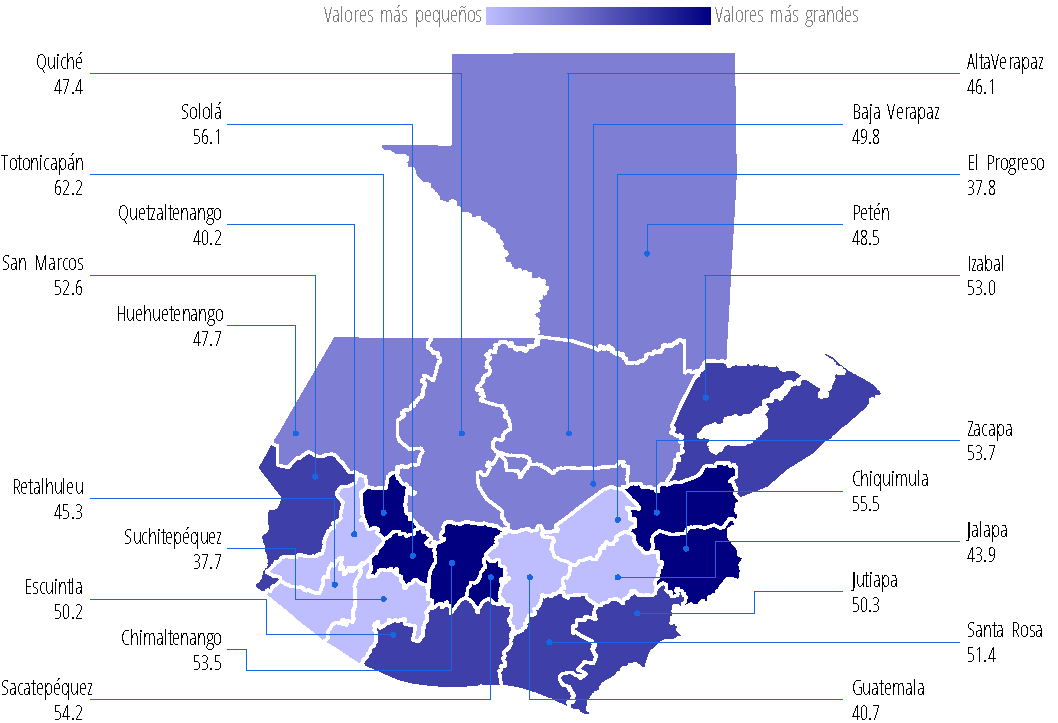
\includegraphics[width=52\cuadri]{graficas/6_09.pdf}}%
{%
	Encuesta Nacional de Salud Materno Infantil (Ensmi), 2008/2009} %
	\INEchaptercarta{Inversión pública en SAN }{La dimensión sobre Inversión Pública en Seguridad Alimentaria y Nutricional tiene como finalidad recabar información sobre los logros alcanzados en materia de SAN en los últimos años para Guatemala. Esta dimensión se compone por un indicador, el cual reúne cinco sub-indicadores.
	}	\begin{figure}[ht]
	\begin{adjustbox}{addcode={\begin{minipage}{\width}}{\caption{%
						Indicadores y subindicadores del capítulo 7. Inversión pública en SAN. 
					} \qquad \qquad \qquad \qquad\qquad \qquad\qquad \qquad\qquad    Elaborado por: Iarna-URL, 2016.\end{minipage}},rotate=90,center}
		\includegraphics[scale=.45]{MapaInversion.jpeg}%
	\end{adjustbox}
\end{figure}
	\cleardoublepage

	%#########################1########################

\stepcounter{section}
\begin{center}
	\textbf{\color{color2} \thesection} \quad  \textbf{Integración del presupuesto en SAN del plan del pacto Hambre Cero a nivel nacional} \addcontentsline{toc}{section}{\numberline{\thesection} Integración del presupuesto en SAN del plan del pacto Hambre Cero a nivel nacional}
\end{center}
$\ $ \\[-5cm]
 \cajita{%
Tasa de Asignación presupuestaria en Seguridad Alimentaria y Nutricional (SAN), del Pacto Hambre Cero (PH0) años 2012 a 2015 }%
{%
	Hambre Cero es un programa social del Gobierno guatemalteco introducido  en 2012 con el objetivo de erradicar la desnutrición crónica infantil y la pobreza extrema.
	
	El Pacto Hambre Cero, busca disminuir en 10\% la prevalencia de la desnutrición crónica en un plazo de 4 años, lo cual será la base para lograr una reducción del 24\% en los próximos 10 años.  En 2015 la tasa de asignación respecto del presupuesto general de la nación fue de 7.7 \%.  
 }%
{%
Tasa de Asignación presupuestaria en Seguridad Alimentaria y Nutricional (SAN), del Pacto Hambre Cero (PH0) respecto del presupuesto general de la nación } %
{%
 República de Guatemala, serie histórica, en porcentaje} %
{%
 \begin{tikzpicture}[x=1pt,y=1pt]  \input{graficas/7_01.tex}  \end{tikzpicture}}%
{%
 Sicoin} %


 \cajita{%
 	Ejecución presupuestaria en Seguridad Alimentaria y Nutricional (SAN), del Pacto Hambre Cero (PH0)}%
 {%
 	
 	
 	La ejecución presupuestaria en Seguridad Alimentaria y Nutricional (SAN), del Pacto Hambre Cero (PH0) entre el 2012 y 2015 ha variado entre 66.6 y 89.2 por ciento, teniendo su ejecuación más baja en el 2015.
 }%
 {%
 	Tasa de ejecución de la Sesan respecto al presupuesto asignado } %
 {%
 	República de Guatemala, serie histórica, en porcentaje} %
 {%
 	\begin{tikzpicture}[x=1pt,y=1pt]  \input{graficas/7_02.tex}  \end{tikzpicture}}%
 {%
 	Sicoin} %
 
 
  \cajita{%
  	Detalle de presupuesto asignado del plan del Pacto Hambre Cero (PPH0) }%
  {%
  	Para atender la desnutrición se implementó el plan hambre cero, siendo la Sesan parte importante en la ejecución del mismo. 
  		
  		En Plan Hambre Cero está compuesto por componentes directos, de viabilidad y el eje transversal, siendo este último el aspecto en el que menos se invirtió dinero por parte del estado para el 2015.
  }%
  {%
  	Detalle de ejecución para el plan del Pacto Hambre Cero (PPH0) } %
  {%
  	República de Guatemala, 2015, en quetzales} %
  {%
  	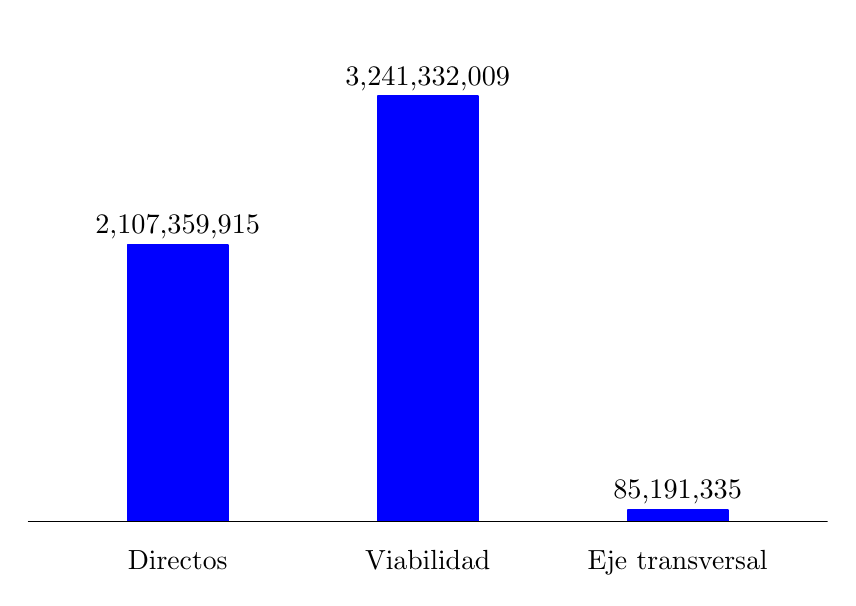
\begin{tikzpicture}[x=1pt,y=1pt]  % Created by tikzDevice version 0.9 on 2016-03-03 06:36:59
% !TEX encoding = UTF-8 Unicode
\definecolor{fillColor}{RGB}{255,255,255}
\path[use as bounding box,fill=fillColor,fill opacity=0.00] (0,0) rectangle (289.08,198.74);
\begin{scope}
\path[clip] (  0.00,  0.00) rectangle (289.08,198.74);

\path[] (  0.00,  0.00) rectangle (289.08,198.74);
\end{scope}
\begin{scope}
\path[clip] (  0.00,  0.00) rectangle (289.08,198.74);

\path[] (  0.00, 12.77) rectangle (289.08,181.67);

\path[] ( 54.20, 12.77) --
	( 54.20,181.67);

\path[] (144.54, 12.77) --
	(144.54,181.67);

\path[] (234.88, 12.77) --
	(234.88,181.67);
\definecolor{drawColor}{RGB}{0,0,255}
\definecolor{fillColor}{RGB}{0,0,255}

\path[draw=drawColor,line width= 0.6pt,line join=round,fill=fillColor] ( 36.13, 20.44) rectangle ( 72.27,120.27);

\path[draw=drawColor,line width= 0.6pt,line join=round,fill=fillColor] (126.47, 20.44) rectangle (162.61,173.99);

\path[draw=drawColor,line width= 0.6pt,line join=round,fill=fillColor] (216.81, 20.44) rectangle (252.95, 24.48);
\definecolor{drawColor}{RGB}{0,0,0}

\path[draw=drawColor,line width= 0.1pt,line join=round] (  0.00, 20.44) -- (289.08, 20.44);

\node[text=drawColor,anchor=base,inner sep=0pt, outer sep=0pt, scale=  1.02] at ( 54.20,124.25) {2,107,359,915};

\node[text=drawColor,anchor=base,inner sep=0pt, outer sep=0pt, scale=  1.02] at (144.54,177.96) {3,241,332,009};

\node[text=drawColor,anchor=base,inner sep=0pt, outer sep=0pt, scale=  1.02] at (234.88, 28.45) {85,191,335};

\path[] (  0.00, 12.77) rectangle (289.08,181.67);
\end{scope}
\begin{scope}
\path[clip] (  0.00,  0.00) rectangle (289.08,198.74);

\path[] (  0.00, 12.77) --
	(289.08, 12.77);
\end{scope}
\begin{scope}
\path[clip] (  0.00,  0.00) rectangle (289.08,198.74);

\path[] ( 54.20, 10.02) --
	( 54.20, 12.77);

\path[] (144.54, 10.02) --
	(144.54, 12.77);

\path[] (234.88, 10.02) --
	(234.88, 12.77);
\end{scope}
\begin{scope}
\path[clip] (  0.00,  0.00) rectangle (289.08,198.74);
\definecolor{drawColor}{RGB}{0,0,0}

\node[text=drawColor,anchor=base,inner sep=0pt, outer sep=0pt, scale=  1.00] at ( 54.20, 3.00) {Directos};

\node[text=drawColor,anchor=base,inner sep=0pt, outer sep=0pt, scale=  1.00] at (144.54, 3.00) {Viabilidad};

\node[text=drawColor,anchor=base,inner sep=0pt, outer sep=0pt, scale=  1.00] at (234.88, 3.00) {Eje transversal};
\end{scope}
  \end{tikzpicture}}%
  {%
  	Sicoin} %
  
  
  
  \cajita{%
  	Asignación presupuestaria a la Ventana de los Mil Días}%
  {%	
  	En la serie histórica se observa que ha habido un aumento en la inversión para el Plan la Ventana de los Mil Días. En el 2015 se hizo una asignación de 705,840,558 quetzales. 
  }%
  {%
  Asignación presupuestaria al programa ventana de los mi días para el año 2015} %
  {%
  	República de Guatemala, serie histórica, en quetzales} %
  {%
  	\begin{tikzpicture}[x=1pt,y=1pt]  \input{graficas/7_04.tex}  \end{tikzpicture}}%
  {%
  	Sicoin} %
  
  
    \cajita{%
    	Gasto Programa Ventana de los Mil Días}%
    {%
    	El Programa  Ventana de los Mil Días tiene varios rubros de inversión.
    	
    	Para el 2015 el gasto se centralizó en la compra de vacunas, seguido de la compra de Vitamina A.
    }%
    {%
    	Detalle del gasto en el Plan Ventana de los Mil Días} %
    {%
    	República de Guatemala, 2015, en miles de millones quetzales} %
    {%
    	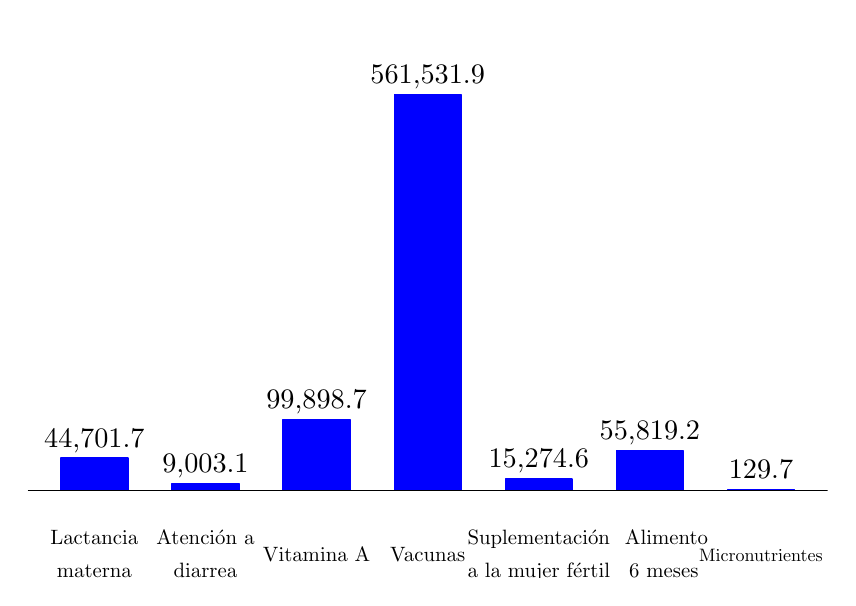
\begin{tikzpicture}[x=1pt,y=1pt]  % Created by tikzDevice version 0.9 on 2016-03-03 06:46:08
% !TEX encoding = UTF-8 Unicode
\definecolor{fillColor}{RGB}{255,255,255}
\path[use as bounding box,fill=fillColor,fill opacity=0.00] (0,0) rectangle (289.08,198.74);
\begin{scope}
\path[clip] (  0.00,  0.00) rectangle (289.08,198.74);

\path[] (  0.00,  0.00) rectangle (289.08,198.74);
\end{scope}
\begin{scope}
\path[clip] (  0.00,  0.00) rectangle (289.08,198.74);

\path[] (  0.00, 24.65) rectangle (289.08,181.67);

\path[] ( 24.09, 24.65) --
	( 24.09,181.67);

\path[] ( 64.24, 24.65) --
	( 64.24,181.67);

\path[] (104.39, 24.65) --
	(104.39,181.67);

\path[] (144.54, 24.65) --
	(144.54,181.67);

\path[] (184.69, 24.65) --
	(184.69,181.67);

\path[] (224.84, 24.65) --
	(224.84,181.67);

\path[] (264.99, 24.65) --
	(264.99,181.67);
\definecolor{drawColor}{RGB}{0,0,255}
\definecolor{fillColor}{RGB}{0,0,255}

\path[draw=drawColor,line width= 0.6pt,line join=round,fill=fillColor] ( 12.04, 31.78) rectangle ( 36.14, 43.15);

\path[draw=drawColor,line width= 0.6pt,line join=round,fill=fillColor] ( 52.20, 31.78) rectangle ( 76.29, 34.07);

\path[draw=drawColor,line width= 0.6pt,line join=round,fill=fillColor] ( 92.35, 31.78) rectangle (116.43, 57.18);

\path[draw=drawColor,line width= 0.6pt,line join=round,fill=fillColor] (132.50, 31.78) rectangle (156.59,174.53);

\path[draw=drawColor,line width= 0.6pt,line join=round,fill=fillColor] (172.64, 31.78) rectangle (196.73, 35.67);

\path[draw=drawColor,line width= 0.6pt,line join=round,fill=fillColor] (212.80, 31.78) rectangle (236.88, 45.97);

\path[draw=drawColor,line width= 0.6pt,line join=round,fill=fillColor] (252.94, 31.78) rectangle (277.03, 31.82);
\definecolor{drawColor}{RGB}{0,0,0}

\path[draw=drawColor,line width= 0.1pt,line join=round] (  0.00, 31.78) -- (289.08, 31.78);

\node[text=drawColor,anchor=base,inner sep=0pt, outer sep=0pt, scale=  1.02] at ( 24.09, 47.12) {44,701.7};

\node[text=drawColor,anchor=base,inner sep=0pt, outer sep=0pt, scale=  1.02] at ( 64.24, 38.04) {9,003.1};

\node[text=drawColor,anchor=base,inner sep=0pt, outer sep=0pt, scale=  1.02] at (104.39, 61.15) {99,898.7};

\node[text=drawColor,anchor=base,inner sep=0pt, outer sep=0pt, scale=  1.02] at (144.54,178.50) {561,531.9};

\node[text=drawColor,anchor=base,inner sep=0pt, outer sep=0pt, scale=  1.02] at (184.69, 39.64) {15,274.6};

\node[text=drawColor,anchor=base,inner sep=0pt, outer sep=0pt, scale=  1.02] at (224.84, 49.95) {55,819.2};

\node[text=drawColor,anchor=base,inner sep=0pt, outer sep=0pt, scale=  1.02] at (264.99, 35.79) {129.7};

\path[] (  0.00, 24.65) rectangle (289.08,181.67);
\end{scope}
\begin{scope}
\path[clip] (  0.00,  0.00) rectangle (289.08,198.74);

\path[] (  0.00, 24.65) --
	(289.08, 24.65);
\end{scope}
\begin{scope}
\path[clip] (  0.00,  0.00) rectangle (289.08,198.74);

\path[] ( 24.09, 21.90) --
	( 24.09, 24.65);

\path[] ( 64.24, 21.90) --
	( 64.24, 24.65);

\path[] (104.39, 21.90) --
	(104.39, 24.65);

\path[] (144.54, 21.90) --
	(144.54, 24.65);

\path[] (184.69, 21.90) --
	(184.69, 24.65);

\path[] (224.84, 21.90) --
	(224.84, 24.65);

\path[] (264.99, 21.90) --
	(264.99, 24.65);
\end{scope}
\begin{scope}
\path[clip] (  0.00,  0.00) rectangle (289.08,198.74);
\definecolor{drawColor}{RGB}{0,0,0}

\node[text=drawColor,anchor=base,inner sep=0pt, outer sep=0pt, scale=  0.750] at ( 24.09, 11.88) {Lactancia };

\node[text=drawColor,anchor=base,inner sep=0pt, outer sep=0pt, scale=  0.750] at ( 24.09,  0.00) {  materna};

\node[text=drawColor,anchor=base,inner sep=0pt, outer sep=0pt, scale=  0.750] at ( 64.24, 11.88) {Atención a };

\node[text=drawColor,anchor=base,inner sep=0pt, outer sep=0pt, scale=  0.750] at ( 64.24,  0.00) { diarrea};

\node[text=drawColor,anchor=base,inner sep=0pt, outer sep=0pt, scale=  0.750] at (104.39,  5.94) {Vitamina A};

\node[text=drawColor,anchor=base,inner sep=0pt, outer sep=0pt, scale=  0.750] at (144.54,  5.94) {Vacunas};

\node[text=drawColor,anchor=base,inner sep=0pt, outer sep=0pt, scale=  0.750] at (184.69, 11.88) {Suplementación};

\node[text=drawColor,anchor=base,inner sep=0pt, outer sep=0pt, scale=  0.750] at (184.69,  0.00) {a la  mujer fértil};

\node[text=drawColor,anchor=base,inner sep=0pt, outer sep=0pt, scale=  0.750] at (230.84, 11.88) {Alimento};

\node[text=drawColor,anchor=base,inner sep=0pt, outer sep=0pt, scale=  0.750] at (229.84,  0.00) { 6 meses};

\node[text=drawColor,anchor=base,inner sep=0pt, outer sep=0pt, scale=  0.650] at (264.99,  5.94) {Micronutrientes};
\end{scope}
  \end{tikzpicture}}%
    {%
    	Sicoin} %
  
	\cleardoublepage
		\input{literatura.tex}
		\appendix


		\input{tablaC1.tex}
		
		\input{tablaC2.tex}
		\input{tablaC3.tex}
		
		\input{tablasC4.tex}
		\input{tablaC5.tex}  %%%sin segunda revision
		\input{tablaC6.tex}  %%%Revisar la nota en la tabla de bajo peso y talla %%%sin segunda revision
		\input{tablaC7.tex}%%%sin segunda revision
	

\end{document}
